\documentclass[lettersize,journal]{IEEEtran}
\usepackage{amsmath,amsfonts}
\usepackage{amssymb}
\usepackage{bigints}
\usepackage{algorithmic}
\usepackage{algorithm}
\usepackage{array}
\usepackage[caption=false,font=normalsize,labelfont=sf,textfont=sf]{subfig}
\usepackage{textcomp}
\usepackage{stfloats}
\usepackage{url}
\usepackage{verbatim}
\usepackage{graphicx}
\usepackage{cite}
\usepackage{pgfplots}
\usepackage{tikz}
\usetikzlibrary{spy}

\hyphenation{op-tical net-works semi-conduc-tor IEEE-Xplore}

\graphicspath{{figures/}}

\begin{document}

\title{Image-based trail bundling for ambiguity avoidance}

\author{Lucas Stankus, Alexandru Telea, and Fabio Kon
\thanks{This paper was produced by the IEEE Publication Technology Group. They are in Piscataway, NJ.}% <-this % stops a space
\thanks{Manuscript received April 19, 2021; revised August 16, 2021.}}

% The paper headers
\markboth{Journal of \LaTeX\ Class Files,~Vol.~14, No.~8, August~2021}%
{Shell \MakeLowercase{\textit{et al.}}: A Sample Article Using IEEEtran.cls for IEEE Journals}

% \IEEEpubid{0000--0000/00\$00.00~\copyright~2021 IEEE}
% Remember, if you use this you must call \IEEEpubidadjcol in the second
% column for its text to clear the IEEEpubid mark.

\maketitle

%!TeX root=../paper.tex

\begin{abstract}
\end{abstract}

\begin{IEEEkeywords}
Ambiguity, Graph, Path, Bundling, Graph Bundling, Path Bundling, Data Visualization.
\end{IEEEkeywords}

%!TeX root=../paper.tex

\section{Introduction}
\label{sec:intro}

\IEEEPARstart{P}{ath} bundling has emerged as a prominent method for reducing visual clutter and highlighting key insights in visualizations of large graph embeddings and trail-sets. Modern path bundling techniques are capable of processing datasets with millions of paths (edges or trails) on consumer hardware, offering a powerful means of visualizing complex data\cite{lhuillier:2017:survey}. However, path bundling introduces distortion and overlap in the visualization. While these techniques can effectively reduce visual clutter, they also risk inducing incorrect interpretations or assumptions about the data. A significant issue associated with path bundling is path ambiguity, where the bundled drawing suggests connections not present in the underlying data.

Despite its prevalence, path ambiguity is not explicitly addressed by most existing bundling methods. Notable techniques such as FDEB\cite{holten:2009}, KDEEB\cite{hurter:2012}, and CUBu\cite{van:2016} all prioritize spatial proximity of paths when creating bundles. While this approach significantly reduces visual clutter, it potentially creates bundles with unrelated paths, exacerbating the ambiguity problem previously described. Grid-based techniques, such as Winding Roads\cite{lambert:2010}, SBEB\cite{ersoy:2011}, and GBEB\cite{cui:2008}, split paths into smaller bundles, which helps maintain path coherence to some extent, but can still introduce ambiguity to the visualization.

Confluent Drawings (CD)\cite{dickerson:2002} address a similar issue by computing both the layout and clustered drawing of a graph. These methods propose strict requirements for edge clustering on the graph structure, which drastically limits ambiguity. However, CDs cannot be applied to all graphs, are computationally expensive, and, because of the rigorous formulation, are less effective at reducing visual clutter than bundling techniques; making CD techniques unsuitable for visualizing large networks.

% Confluent Drawings (CD)\cite{dickerson:2002} address a similar issue by computing both the layout and clustered drawing of a graph. These methods propose strict requirements for edge clustering based on the network structure and, by design, do not introduce ambiguity to the drawing. However, this approach is computationally expensive and, because of the rigorous formulation, less effective at reducing visual clutter than bundling techniques; making CD techniques unsuitable for visualizing large networks.

% Edge-Path Bundling (EP)\cite{wallinger:2022} attempts to fit in the middle ground between standard bundling and CD techniques. EP creates bundles using network structure with looser rigidity compared to CD techniques, removing what they define as \emph{independent edge ambiguity} by design. However, EP approach introduces significant spatial distortion compared to the original drawing, which can introduce other types of ambiguities in the visualizations. The distortion also limits EP's effectiveness in applications where preserving the spatial information of embeddings is crucial, such as mobility data visualization.

Given the shortcomings on CD techniques, hybrid approaches between path bundling and CD emerged to fit the gap between them, providing less ambiguous bundling\cite{bach:2016,zheng:2021,wallinger:2022}. However, regardless of these advancements, there remains a critical gap in the field: the need for a method that effectively reduces visual clutter while simultaneously minimizing edge ambiguity, especially when the spatial embeddings encode crucial information. Current approaches often sacrifice one aspect for the other, leaving room for significant improvement in balancing these competing objectives.

% NOTE:
% Lucas: Edge-Path tries to fill this gap, but I think we can argue that it does not fit well here. Even though its whole proposition is to remove independent edge ambiguities by design, it performs kinda similar to other methods in terms of ambiguity (using their own metric); and much worse using our own ambiguity metric. Thus I think we can argue that no such method exists currently. Our proposition (as seen in later examples) heavily reduces ambiguities by sacrificing clutter reduction, but is still much much better than confluent drawings (all according to our metric).

In this paper, we propose a novel approach for reducing visual clutter with minimal path ambiguity. Our contributions are fourfold: First, we introduce a new image-based metric for quantifying ambiguity at a local level throughout the drawing, providing pixel-level ambiguity values. Second, we propose an extension applicable to any iterative bundling technique to minimize ambiguity, utilizing our metric to constrain ambiguous bundle formation without altering the underlying algorithm. Third, we present an implementation of our approach using the CUBu framework, demonstrating an ambiguity-avoiding bundling technique. Fourth, we provide an open-source reproducibility package containing the code and data used in this paper.

The remainder of this paper is organized as follows: Section \ref{sec:rw} reviews related work on edge bundling. Section \ref{sec:ambiguity} introduces our metric for quantifying ambiguity. Section \ref{sec:bundling} details our method for enhancing iterative bundling techniques with ambiguity avoidance. Section \ref{sec:experiments} presents applications of our bundling method. Section \ref{sec:discussion} analyzes the key aspects of our metric and method. Section \ref{sec:limitations} addresses limitations of our work. Finally, Section \ref{sec:conclusion} summarizes our findings and concludes the paper.

%!TeX root=../paper.tex

\section{Related Work}\label{sec:rw}

% lucas: Not sure if it is okay to start directly with these subsections or not

Building upon our contributions described in Section \ref{sec:intro}, we review existing literature on path bundling and ambiguity measurements and avoidance.

% I couldn't think of a way to properly split edge bundling from trial bundling (and consequently path
% bundling with the combination of both) that wouldn't make this paragraph too long.
\textbf{Path bundling:} Since the introduction of edge bundling by Holten\cite{holten:2006}, numerous techniques emerged to bundle both graph drawings and trail-sets\cite{lhuillier:2017:survey}. Edge and trail bundling techniques, which we can globally denote as path bundling, aim to group paths by their spatial similarity and, optionally, their data and general network structure. Path bundling can be done using control-meshes\cite{cui:2008}, quadtrees for spatial-partitioning\cite{lambert:2010}, force-directed algorithms\cite{holten:2009,nguyen:2012,selassie:2011}, and multilevel ink-saving clustering\cite{gansner:2011}. Along them, image-based techniques\cite{telea:2010,ersoy:2011,hurter:2012,bottger:2014,wu:2015,van:2016,lhuillier:2017:ffteb,zeng:2019} operate on the pixels of path to leverage the GPU for scalability. While these methods are the most efficient, being able to bundle datasets with millions of paths, they often sacrifice fine control over bundle formation for performance.

The current state-of-the-art bundling methods group paths almost exclusively on spatial proximity. As such, these methods are all affected by \emph{path ambiguity} issues. While the proper definition of path ambiguity varies in the literature, in essence, ambiguity arises when there is loss of information about the connectivity patterns of the network. When there is ambiguity, users can be misled by the visualization and perceive false adjacencies or incorrect relationships between nodes. This leads to misinterpretation and wrong assumptions about the underlying data and structures. There have been works that aim to mitigate ambiguity in bundled drawings, however ambiguity is a complicated issue. When designing a bundling algorithm, one needs to mitigate three opposing forces:

\begin{enumerate}
\item \textbf{Removal of visual clutter:} Visual complexity of the image should be kept at a minimum.
\item \textbf{Ambiguity-avoidance:} The user's understanding of the underlying connectivity should be preserved.
\item \textbf{Geometric closeness to the original input:} Distortion of the original data should not be too extreme.
\end{enumerate}

These forces interact in complex ways. For instance, if one takes \#1 to the extreme and bundles too extensively, the amount of distortion necessary would likely break \#3 and make it difficult to maintain \#2, as paths with drastically different connectivity would be bundled together, leading to false adjacencies. On the other hand, prioritizing \#2 or \#3 too extensively might lead to bundled drawings with excessive visual clutter. This tension highlights the fundamental challenge in designing effective bundling algorithms that must balance these competing factors.

% lucas: Complexity analysis here is actually NP-completeness, don't know if we should mention it.
\textbf{Confluent Drawings (CD):} Introduced by Dickerson \textit{et al.}\cite{dickerson:2002}, CDs do not tackle the exact same problem as edge bundling but face similar issues. The core idea behind CD is the strict use of the graph network to create confluent bundles, where only edges from $K_{n,m}$ subgraphs can be grouped. As from the original proposition, CDs are also crossing-free; therefore not every graph has a valid confluent drawing. Different CD techniques have been proposed from a theoretical point of view\cite{eppstein:2006,hui:2007,eppstein:2013}, with considerations on their mathematical formulation and complexity analysis. Other works propose algorithms for CD variations, typically tackling both the graph layout problem and the clusterization of edges\cite{dickerson:2002,hirsch:2007,eppstein:2007,honciuc:2009}; this differentiates them from path bundling, which requires a layout as input. The strict requirements from CDs virtually eliminate ambiguity; however, following the bundling balancing act, the strong ambiguity-avoidance implies they cannot reduce visual clutter as extensively as bundling techniques.

\textbf{Ambiguity-avoidance:} As most bundling techniques converged to bundle based on spatial proximity, some approaches took inspiration from CDs to move towards less ambiguous path bundling. Selassie \textit{et al.}\cite{selassie:2011} presented a modified FDEB algorithm, incorporating directionality and structural information to improve bundle formation. Luo \textit{et al.}\cite{luo:2012} used a combination of spatial-partitioning, congestion metrics, and deformation of edges in what they defined as ambiguity-free edge bundling. Nocaj and Brandes\cite{nocaj:2013} forced cohesive edge angles near endpoints and minimal bends to avoid ambiguity on undirected graphs and introduced confluent spiral drawings for directed graphs. Hybrid techniques between CD and path bundling also emerged. Most notably, Bach \textit{et al.}\cite{bach:2016} used power-graphs as a base and used the new hierarchy to both draw and bundle the graph. Their approach was later improved by Zheng \textit{et al.}\cite{zheng:2021} to create power-confluent drawings with minimal edge crossings. All these approaches were important advances towards less ambiguous bundling, but they still suffer drastically with visual clutter compared to other state-of-the-art bundling techniques.

Finally, Wallinger \textit{et al.}\cite{wallinger:2022} proposed Edge-Path bundling (EP), a hybrid technique that uses weighted paths for bundling. Edge-Path groups long edges along the shorted path made from smaller edges, grouping edges solely on existing connections. Their work also expands the concept of edge ambiguity by categorizing it into three types: \emph{independent-edge ambiguity}, when edges with independent endpoints are bundled; \emph{path endpoint ambiguity}, when subsequent node connections lead to misinterpretation on how far connections extend within the chain; and \emph{path crossing ambiguity}, when shallow crossing angles create misinterpretation of the connectivity patterns. According to their classification, EP focuses on eliminating independent edge ambiguities.

Building on EP's ambiguity definition, we further expand this concept. Previously, ambiguity has been analyzed from the perspective of graph structure, where the only source of truth is the network structure itself. However, when considering a layout, the spatial encoding typically carries information about the data and relationships. Layouts are also cautiously crafted, as even simple design decisions, such as the distance between nodes, can influence users' interpretations\cite{mcgrath:1996,fabrikant:2008}. We propose that path ambiguity should not be treated as a binary concept, where all false connections carry equal weight. Instead, we consider false connections between similar structures, such as individual nodes within two heavily linked clusters, as less ambiguous than those between entirely unrelated regions.

\textbf{Ambiguity quality metrics:} Together with visualization tools, there has been significant advances in measuring the quality of said visualizations. Several works emerged to measure various aspects of graph visualization, including edge congestion\cite{carpendale:2001}, entropy\cite{tufte:1983}, faithfulness\cite{nguyen:2013,nguyen:2017}, readability\cite{dunne:2009,dunne:2015}, and entropy\cite{sips:2009,tatu:2009}. Despite that some of these metrics indirectly measured ambiguity, few works have ambiguity as a focus. Edge-Path\cite{wallinger:2022} presents a graph quality metric for ambiguity based on faithfulness, using the proportion of true and false connections. AmbiguityVis\cite{wang:2016} introduces several metrics tailor-made to measure ambiguity and displays them in a heatmap for users, allowing them to check for misleading areas. However, both of them have strict focus on graph structure, failing to consider the spatial layout. We propose a new metric that considers the spatial layout, aiming to provide a more comprehensive view of ambiguity in path bundling.

%!TeX root=../paper.tex

\section{Measuring Ambiguity}\label{sec:ambiguity}

Based on the expanded concept of path ambiguity introduced in the previous section, we propose a novel metric to evaluate ambiguity in bundled visualizations. Since bundling methods do not generate drawings from the original data, they operate on a given input drawing. Our metric aims to take the input drawing into account and incorporate the information from these spatial embeddings into the ambiguity calculation. To our knowledge, this is the only ambiguity metric that can compute ambiguity for both graph drawings and trail-sets, making it the first comprehensive path-ambiguity metric.

Our metric introduces two key contributions. First, we propose a spatially-aware approach that computes local ambiguity values throughout the drawing, providing detailed insight into problematic regions instead of reducing ambiguity to a single global value. Second, we introduce a continuous approach to crossing ambiguity that considers the similarity between overlapping paths, moving beyond the traditional binary classification of ambiguous crossings. These contributions enable a more nuanced evaluation of bundled visualizations while accounting for their spatial characteristics.

While the ambiguities presented in Edge-Path focus exclusively on edge bundling, they can be adapted to general path bundling. Edge-crossing ambiguities and path endpoint ambiguities remain unchanged, as they still introduce the same incorrect assumptions. Independent-edge ambiguities are also present, but instead of relying solely on individual vertices to trigger this ambiguity, we consider the spatial encodings of the endpoints; for example, by considering whether the vertices belong to the same cluster.

Next, we formalize these concepts into a metric that captures both the structural and spatial aspects of path ambiguity.

% ------- SUBSECTION -------

\subsection{Proposed metric}

Let $\mathcal{D}$ be the space of all possible drawings and $D(P) = \{p_i \subset \mathbb{R}^2 \}$ be a drawing of a path-set $P$, where $p_i$ can be either a straight line, for graph drawings, or a curve in space, for trail-sets. Let $B: \mathcal{D} \rightarrow \mathcal{D}$ be a general bundling operator, we formalize that a pair of paths $p_i \in D(P)$ and $B(p_j) \in B(D(P))$ as being counterparts of each other when $p_i$ generates $p_j$ after the bundling operator $B$ is applied to $D_G$. Finally, we define the metric as a scalar field $\omega : \mathbb{R}^2 \rightarrow \mathbb{R}_{+}$ that represents ambiguity throughout the drawing.

Before delving into the technical details, we present a high-level overview of $\omega$ formulation. First, we take all $B(p_i) \in B(D(P))$ that intersect a neighborhood and select their counterparts in $D(P)$. We then take the average distance between all possible pairs of the selected paths. Additionally, we apply both a convolution and a normalization steps to the scalar field to smooth the resulting values. 

We argue that the comparison between paths in $B(D(P))$ and their original counterparts in $D(P)$ bridges the gap between both drawings, providing an estimate of bundle formation quality throughout the bundled drawing. We now present how $\omega$ is defined for a given location $\mathbf{x} \in \mathbb{R}^2$, detailing each step of its calculation: (1) the selection of paths and their counterparts, (2) the distance calculations between paths, (3) the convolution, and (4) the normalization process.

% --- step 1:

\textbf{Selection of paths and counterparts (step 1):}
% lucas: I was naming the two user defined parameters with rho for consistency and easy identification of parameters vs constants, but it following the email I changed it to simply r, m, and c.
The first step involves selecting the paths from $B(D(P))$ that affect ambiguity at point $\mathbf{x} \in \mathbb{R}^2$. Given a user-defined parameter $r \in \mathbb{N}$, we identify all paths $B(p_i) \in B(D(P)), B(p_i) \cap N_r(\mathbf{x}) \neq \varnothing$, that intersect a neighborhood $N_r(\mathbf{x})$ of radius $r$ and center $\mathbf{x}$. For each intersecting path, we collect the corresponding counterparts from $D(P)$ and group them in the set $\bar{P}_{\mathbf{x}} \in D(P)$.

% --- step 2:

\textbf{Path distances calculation (step 2):}
With the set $\bar{P}_p$ defined, we take the average of the distances between all pairs in $\bar{P}_p$. We define a distance function $\lambda : D(P) \times D(P) \rightarrow \mathbb{R}_{+}$ as a modified weak \emph{Fr\'echet distance}. Let $| p_i |$ be the cardinality of $p_i \in D(P)$, $\| p_i - p_j \|$ be the Euclidean distance between $p_i, p_j \in D(P)$, and $T : \mathbb{R}^2 \rightarrow \mathbb{R}^2$ be a function that returns the tangent of $p_i \in D(P)$ at a given point $\mathbf{a} \in p_i$, we define $\lambda$ defined as follows:

% lucas: if I got the email right, the denominator there is wrong. In the discrete version, we do not divide by the length of the curve, we divide by the number of control point inside it. That is, if we have n sample distances from a to b, we divide the sum of the distances by n. So, I believe here we should divide by the cardinality of p_i here, but I might be completely off.
\begin{equation}
\lambda(p_i, p_j) =
\bigintsss_{\mathbf{a} \in p_i} \frac
{\displaystyle \min_{\mathbf{b} \in p_j} \big(\| \mathbf{a} - \mathbf{b} \|\big) \big(T(\mathbf{a}) \cdot T(\mathbf{b})\big)^2}
{|p_i|}
ds
\end{equation}

By swapping the minimum ``leash'' from the weak \emph{fr\'echet distance}, we make the function less susceptible to drastic changes from outliers. Taking the case depicted in Figure \ref{fig:frechet_example}, the two paths are similar to each other but have a small detour in the middle. With the weak \emph{fr\'echet distance}, this detour drastically alters the resulting distance. However, since these paths share similar endpoints and roughly the same shape, a smaller distance is more desirable. By taking the average, we successfully achieve this, making $\lambda$ better suited for our needs.

\begin{figure}[ht]
\centering
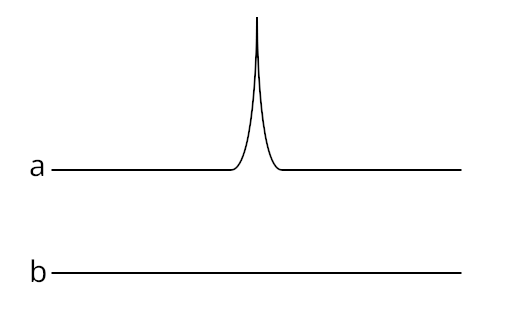
\includegraphics[width=0.48\linewidth]{frechet-example.png}
\caption{Example of case where the weak \emph{fr\'echet distance} is not ideal.}
\label{fig:frechet_example}
\end{figure}

Another critical aspect is the square of the dot product between the tangents of $p_i, p_j \in D(P)$. This dot product reduces the contribution of paths that intersect at near-perpendicular angles, aligning with the edge-crossing ambiguity principle discussed earlier. Squaring the term ensures smooth, differentiable modulation while preventing negative values, preserving the stability and interpretability of $\lambda$.

The distance function $\lambda$ is the core of $\omega$; however, only using the average of distances may generate undesirable results in some datasets. To avoid any issues, we can modulate $\lambda$ with user-defined parameters. We define two functions to modulate $\lambda$ based on the distance from the endpoints of the path and the distance of the path from $\mathbf{x}$. Next, we discuss both the issues that may arise and the modulating functions themselves.

% - distance from endpoints:

\emph{Modulating by distance from endpoints:}
Vertex-adjacent regions in graph drawings often exhibit a higher path density, as multiple paths originate from or terminate at these regions. This concentration leads to large $\bar{P}_{\mathbf{x}}$ sets at those regions and, in certain datasets, results in ambiguity being disproportionately concentrated in vertex clusters. Figure \ref{fig:imbalance_problem} exemplifies this pattern, with ambiguity color-coded from blue to red in increasing ambiguity values. However, we argue that the most problematic regions for path ambiguity tend to be along the middle sections of paths, rather than at their endpoints, since these areas lack the inherent structural context provided by the endpoints.

\begin{figure}[ht]
\centering
\subfloat[$\lambda$ without modulation.]{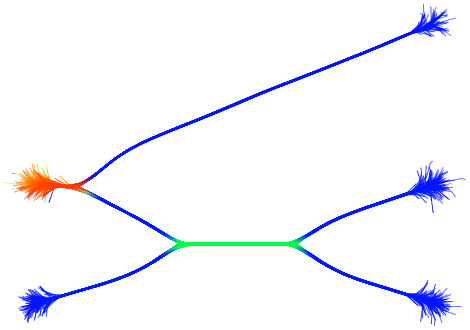
\includegraphics[width=0.48\linewidth]{imbalance-problem.png}\label{fig:imbalance_problem}}
\subfloat[$\lambda$ with $\beta$ modulation.]{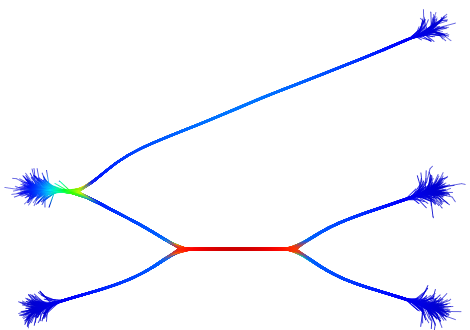
\includegraphics[width=0.48\linewidth]{imbalance-solution.png}\label{fig:imbalance_solution}}\\
\caption{Example of ambiguity concentration on endpoints of $\lambda$, with (b) and without (a) $\beta$ modulation.}
\end{figure}

% lucas: there is probably a more elegant way to describe this, but I couldn't figure it out.
To address this issue, we introduce a modulation function $\beta_{\mathbf{x}} : B(D(P)) \rightarrow [0, 1]$ that weights each path's ambiguity contribution based on its position relative to endpoints. Given a user-defined parameter $m \in [0, \frac{1}{2}[$, $\beta_{\mathbf{x}}$ smoothly transitions from zero near the endpoints to its maximum value in the interval $[m, 1 - m]$. The function uses the normalized arc-length parameter of $B(p_i) \in B(D(P))$ that is closest to $\mathbf{x}$. While the specific formulation of $\beta_{\mathbf{x}}$ is flexible, it should follow the general shape shown in Figure \ref{fig:beta}, where the x-axis represents the normalized position along the path.

\begin{figure}[ht]
\begin{tikzpicture}[scale=1.0]
\begin{axis}[
    axis x line=center,
    axis y line=center,
    x label style={at={(axis description cs:.5,-0.05)},anchor=north},
    y label style={at={(axis description cs:-0.1,.5)},rotate=90,anchor=south},
    xlabel = {Normalized arc-length parameter.},
    ylabel = {$\beta_{\mathbf{x}}$},
    xtick={0},
    ytick={0, 0.5, 1.0},
    xmin=-0.1, xmax=4.6,
    ymin=-0.15, ymax=1.1,
]

\addplot [red, domain=0:1.2  ] { 0.5 - (cos(x         * 48 * pi) / 2) }; 
\addplot [red, domain=1.2:2.8] {  1 };           
\addplot [red, domain=2.8:4  ] { 0.5 - (cos((x - 1.6) * 48 * pi) / 2) }; 

\draw [dashed] (axis cs:1.2,\pgfkeysvalueof{/pgfplots/ymin}) -- (axis cs:1.2,\pgfkeysvalueof{/pgfplots/ymax});
\draw [thick, <->] (axis cs:0,-0.05) -- (axis cs:1.2,-0.05) node[pos=0.5, below] {$m$};

\draw [dashed] (axis cs:2.8,\pgfkeysvalueof{/pgfplots/ymin}) -- (axis cs:2.8,\pgfkeysvalueof{/pgfplots/ymax});
\draw [thick, <->] (axis cs:2.8,-0.05) -- (axis cs:4,-0.05) node[pos=0.5, below] {$m$};

\end{axis}
\end{tikzpicture}
\caption{Graph with the expected shape of $\beta_{\mathbf{x}}$.}
\label{fig:beta}
\end{figure}

We can see the results of applying the $\beta_p$ function in Figure \ref{fig:imbalance_solution}. The modulation effectively shifts the focus of ambiguity from the vertex-adjacent regions to the middle sections of the paths, as intended. This redistribution of ambiguity aligns with our earlier assertion that the most problematic regions typically occur along the middle of path paths rather than at their endpoints.

% - distance from x:

\emph{Modulating by distance from $\mathbf{x}$}:
Another issue present in the initial $\lambda$ formulation is the discontinuity in the scalar field. Using $\mathbf{x}$ as a reference point, as paths approach $N_r(\mathbf{x})$, their proximity is not captured by $\lambda$; when these approaching paths start to intersect $N_r(\mathbf{x})$, they are then included in $\bar{P}_{\mathbf{x}}$ with full weight. This abrupt change in the calculation of $\lambda$ creates discontinuities in the scalar field at the neighborhood's boundary. This is exemplified in Figure \ref{fig:linearity_problem}, where the ambiguity sharply transitions from low (blue) to high (red) in the central region.

\begin{figure}[ht]
\centering
\subfloat[$\lambda$ without modulation.]{
    \begin{tikzpicture}[spy using outlines={circle,red,magnification=3.5,size=2.5cm, connect spies}]
    \node {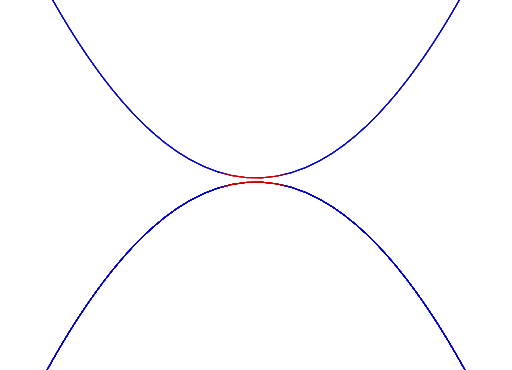
\includegraphics[width=.40\linewidth]{linearity-problem.png}};
    \spy on (0,.05) in node [left] at (2.2,1.7);
    \end{tikzpicture}
    \label{fig:linearity_problem}
}
\subfloat[$\lambda$ with $\alpha$ modulation.]{
    \begin{tikzpicture}[spy using outlines={circle,red,magnification=3.5,size=2.5cm, connect spies}]
    \node {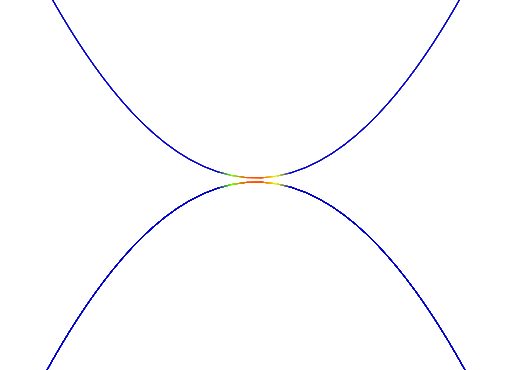
\includegraphics[width=.40\linewidth]{linearity-solution.png}};
    \spy on (0,.05) in node [left] at (2.2,1.7);
    \end{tikzpicture}
    \label{fig:linearity_solution}
}\\
\caption{Example of discontinuity in ambiguity from $\lambda$, with (b) and without (a) $\alpha$ modulation.}
\end{figure}

To address this, we define another modulating function $\alpha_{\mathbf{x}} : B(D(P)) \rightarrow [0,1]$ that smoothly weights the influence of paths on $\lambda$ as they approach $\mathbf{x}$. Specifically, $\alpha_{\mathbf{x}}$ smoothly decreases from 1 to 0 as the Euclidean distance between $\mathbf{x}$ and the closest point on $B(p_i) \in B(D(P))$ increases from 0 to $r$. Similar to $\beta_{\mathbf{x}}$, the specific formulation of $\alpha_{\mathbf{x}}$ is flexible, with Figure \ref{fig:alpha} showing its general shape, where the x-axis represent the distance from $p_i$ to $\mathbf{x}$.

Figure \ref{fig:linearity_solution} demonstrates the effect of applying $\alpha_{\mathbf{x}}$ to modulate $\lambda$. The visualization shows a smooth transition in ambiguity levels from high (red) through medium (yellow) to low (blue), confirming that the modulating function successfully eliminates the sharp discontinuities from the scalar field.

\begin{figure}[h]
\centering
\begin{tikzpicture}[scale=1.0]
\begin{axis}[
    axis x line = center,
    axis y line = left,
    x label style={at={(axis description cs:.5,-0.05)},anchor=north},
    y label style={at={(axis description cs:.05,.5)},rotate=0,anchor=south},
    xlabel = {Distance of path from $\mathbf{x}$},
    ylabel = {$\alpha_{\mathbf{x}}$},
    xtick={0},
    ytick={0, 0.5, 1.0},
    xmin=0, xmax=1.6,
    ymin=-0.15, ymax=1.1,
    trig format plots=rad,
]

\addplot [red, domain=0:1]{0.5*(1+cos(pi*x))}; 
\addplot [red, domain=1:\pgfkeysvalueof{/pgfplots/xmax}] {0}; 

\draw [dashed] (axis cs:1,\pgfkeysvalueof{/pgfplots/ymin}) -- (axis cs:1,\pgfkeysvalueof{/pgfplots/ymax});
\draw [thick, <->] (axis cs:0,-0.05) -- (axis cs:1,-0.05) node[pos=0.5, below] {$r$};

\end{axis}
\end{tikzpicture}
\caption{Graph with expected shape of $\alpha_{\mathbf{x}}$.}
\label{fig:alpha}
\end{figure}


With the modulating functions defined, we have a formulation for ambiguity given by $\gamma : \mathbb{R}^2 \rightarrow \mathbb{R}_{+}$, as follows:

\begin{equation}
\gamma(\mathbf{x} \in \mathbb{R}^2) = \sum_{p_i, p_j \in \bar{P}_{\mathbf{x}}}
\alpha_{\mathbf{x}}(p_i) \beta_{\mathbf{x}}(p_i) \lambda(p_i, p_j)
\end{equation}


% --- step 3:

\textbf{Convolution and normalization (steps 3 and 4):}
Given the scalar field defined by $\gamma$, we apply two final processing steps to optimize $\gamma$ for practical applications. While the modulating functions in $\gamma$ provide initial smoothness, we introduce a convolution step with an Epanechnikov kernel\cite{epanechnikov:1969} $K$ of radius $r$ to guarantee continuity across the entire field. This effectively eliminates potential discontinuities while preserving the essential characteristics of the ambiguity measure.

Following the convolution, we apply a normalization step to ensure field values remain in a consistent range. This normalization can be performed either relative to the existing maximum value in the scalar field, enabling in-dpeth comparison between regions of the same drawings, or through a limiting function, allowing cross-drawing comparisons. Given a user-defined paramter $c \in \mathbb{R}_{+}$, the limiting function is defined as follows:

% lucas: both the division by r^3 and the multiplication by 500 are to make the visualizations behave nicely when we change r. With this configuration, one might leave c at 1.0 and have generally good results across multiple r values. I don't know how to properly explain this in mathematical terms.
\begin{align}
t &= {\displaystyle \gamma(\mathbf{y}) \frac{500c}{r^3}}
\\
f(\mathbf{y} \in \mathbb{R}^2) &= 1 - \frac{1}{e^t}
\end{align}

By constraining $\gamma$ values, the limiting function makes bundle evaluation more stable and reliable when comparing different bundling techniques. This ensures that the scalar field can be used consistently to aid in bundle formation. To maintain visual consistency of the resulting bundles across varying $r$, the $\gamma$ is scaled by $500/r^3$. This scaling compensates for ambiguity growth with $r$, allowing for good visual results with $c = 1$ across different $r$ values.

Finally, we can define $\omega$ with the following equation:

\begin{equation}
\omega(\mathbf{x} \in \mathbb{R}^2) = \int_{\mathbf{y} \in \mathbb{R}^2}K(\|\mathbf{y} - \mathbf{x}\|)f(\mathbf{y})
\end{equation}

% ------- SUBSECTION -------

\subsection{Approximation Techniques}

Computing $\omega$ in real time presents significant challenges. Straightforward GPU implementations face two main issues. First is the compute time: calculating the distances for every pair of paths found throughout all $\bar{P}_p$ sets on-the-fly is computationally expensive. While this issue can be mitigated by pre-computing all pairwise distances, it comes at the cost of increased video memory (VRAM usage. The second issue is the high VRAM consumption required to store every $\bar{P}_p$ set of the drawing. In this case, the mitigations for the first issue clash directly with the second issue, as VRAM consumption quickly becomes too big for consumer hardware.

To address both of these issues, we developed an approximation approach that limits the size of the $\bar{P}_p$ sets by taking a random sub-sample. Our experiments indicate that limiting each set to a maximum of 100 paths preserves $\omega$ precision while drastically reducing VRAM consumption. This approach enables real-time calculation of $\omega$ on consumer-grade GPUs, with memory usage up to an order of magnitude lower compared to the non-approximated version. The random sub-sampling is performed using a simple reservoir sampling technique\cite{vitter:1985}.

% lucas: I have this almost ready from the qualification exam. Just needs to be adapted.
While this approximation introduces a slight trade-off between accuracy and memory efficiency, our experiments show that the impact on accuracy is negligible for most practical applications. The detailed validation for this approximation, including error analysis, can be found in the supplementary material.

% ------- SUBSECTION -------

\subsection{Validation}

Validating a new metric is always challenging, especially when there are no established standards for comparison. As discussed previously, $\omega$ introduces two novel contributions to ambiguity measurement: (1) local ambiguity values for the entire drawing instead of a single global value, and (2) a non-binary operator for crossing paths, where the ambiguity is modulated by the similarity of overlapping paths. Given this novel approach, we validate $\omega$ through a series of qualitative test cases with increasing complexity, demonstrating its effectiveness and reliability. All examples are of bundled drawings using the state-of-the-art CUBu framework\cite{van:2016}.

We begin with the simplest example: two pairs of connected clusters with a single crossing region, as demonstrated in Figure \ref{fig:validation_simple:straight}. In the bundled visualization (Figure \ref{fig:validation_simple:ambiguity}), tracing the original connectivity patterns of the clusters becomes impossible, as all paths converge into a single, ambiguous bundle in the center. This bundle obscures the original connections, creating ambiguity in the visualization. An effective ambiguity metric should reflect this situation by assigning higher values in the central bundle, where ambiguity is high, and lower values to areas where meaning is preserved. $\omega$ successfully captures this pattern, as seen in Figure \ref{fig:validation_simple:ambiguity}. Values are colored from blue (low ambiguity) to yellow (medium ambiguity) to red (high ambiguity), a scheme used consistently in all following test cases.

\begin{figure}[ht]
\centering
\subfloat[Input drawing]{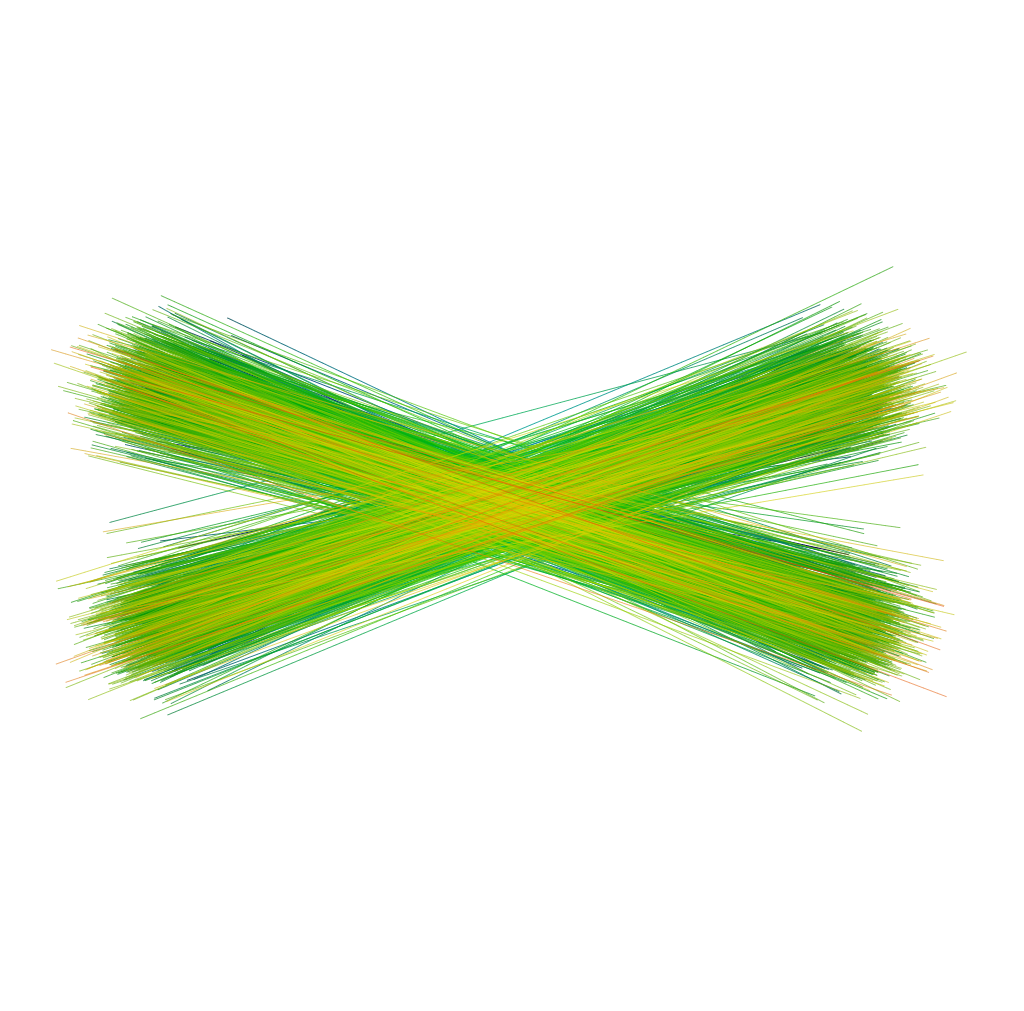
\includegraphics[width=0.48\linewidth]{metric_validation/1_straight.png}\label{fig:validation_simple:straight}}
\subfloat[Bundled drawing]{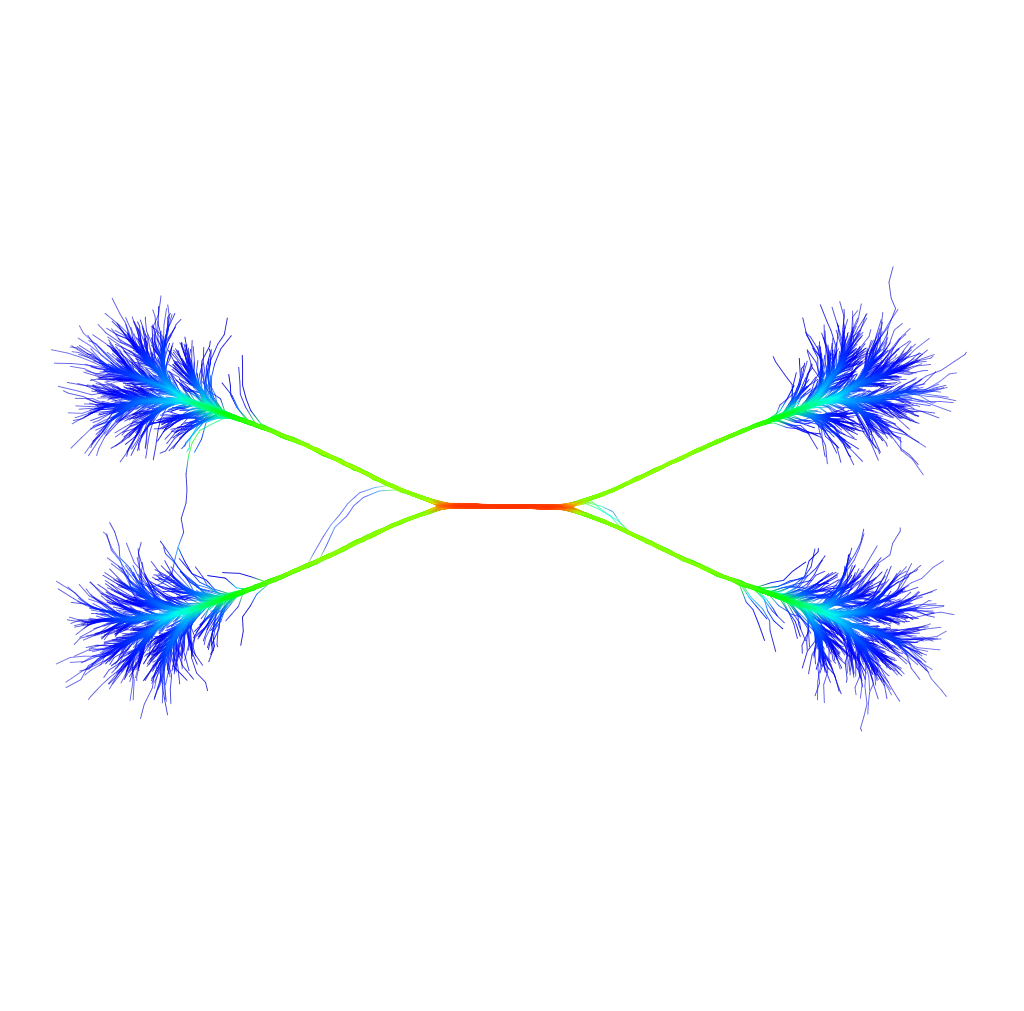
\includegraphics[width=0.48\linewidth]{metric_validation/1_bundled.png}\label{fig:validation_simple:ambiguity}}\\
\caption{Simple example of $\omega$ validation.}
\end{figure}

For a more complex example, we examine three pairs with three crossing regions, as depicted in Figure \ref{fig:validation_medium:straight}. Again, the bundled visualization (Figure \ref{fig:validation_medium:ambiguity}) obfuscates the connectivity patterns in the crossing regions, with multiple paths converging into the same bundle. However, this example introduces additional complexity through its crossing patterns. There are two ambiguous crossings and one non-ambiguous crossing, where the crossing is almost perpendicular. A robust ambiguity metric should correctly identify which of are the ambiguous crossings; which, as shown in Figure \ref{fig:validation_medium:ambiguity}, $\omega$ correctly does with the areas highlighted in red.

\begin{figure}[ht]
\centering
\subfloat[Input drawing]{
\includegraphics[width=0.48\linewidth]{metric_validation/2_straight.png}\label{fig:validation_medium:straight}}
\subfloat[Bundled drawing]{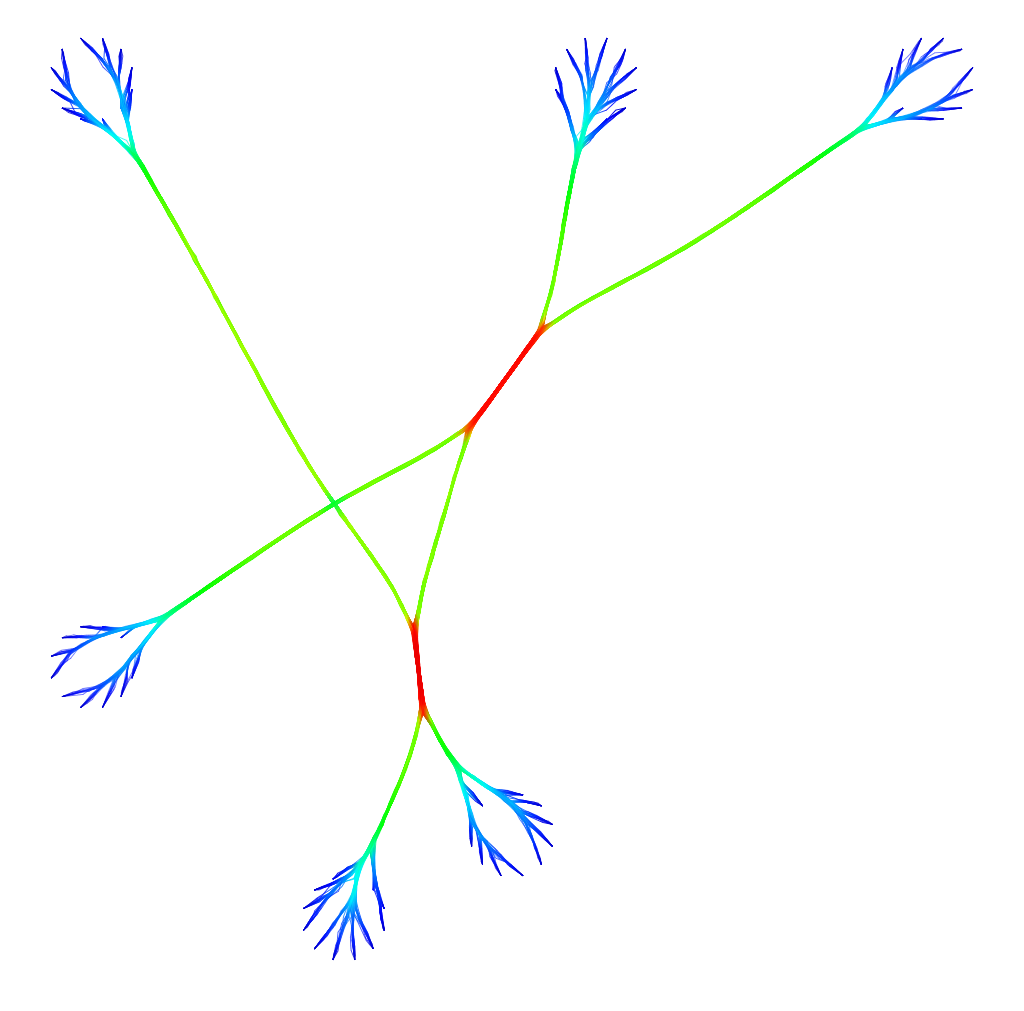
\includegraphics[width=0.48\linewidth]{metric_validation/2_bundled.png}\label{fig:validation_medium:ambiguity}}\\
\caption{Example of $\omega$ validation with perpendicular crossing paths.}
\end{figure}

For our next validation case, we examine when bundles overlap vertex clusters, as depicted in Figure \ref{fig:validation_overlap:straight}. In Figure \ref{fig:validation_overlap:ambiguity}, clusters are connected to multiple clusters instead of only one to one. Additionally, the bundles cross two of the central clusters. However, these overlaps should not be marked with high ambiguity, as it preserves the connectivity patterns of the original network. $\omega$ performs as expected, preserving low to medium ambiguity values in the mentioned bundles, while still highlighting as red the ambiguous cluster in the left side of Figure \ref{fig:validation_overlap:ambiguity}.

\begin{figure}[ht]
\centering
\subfloat[Input drawing]{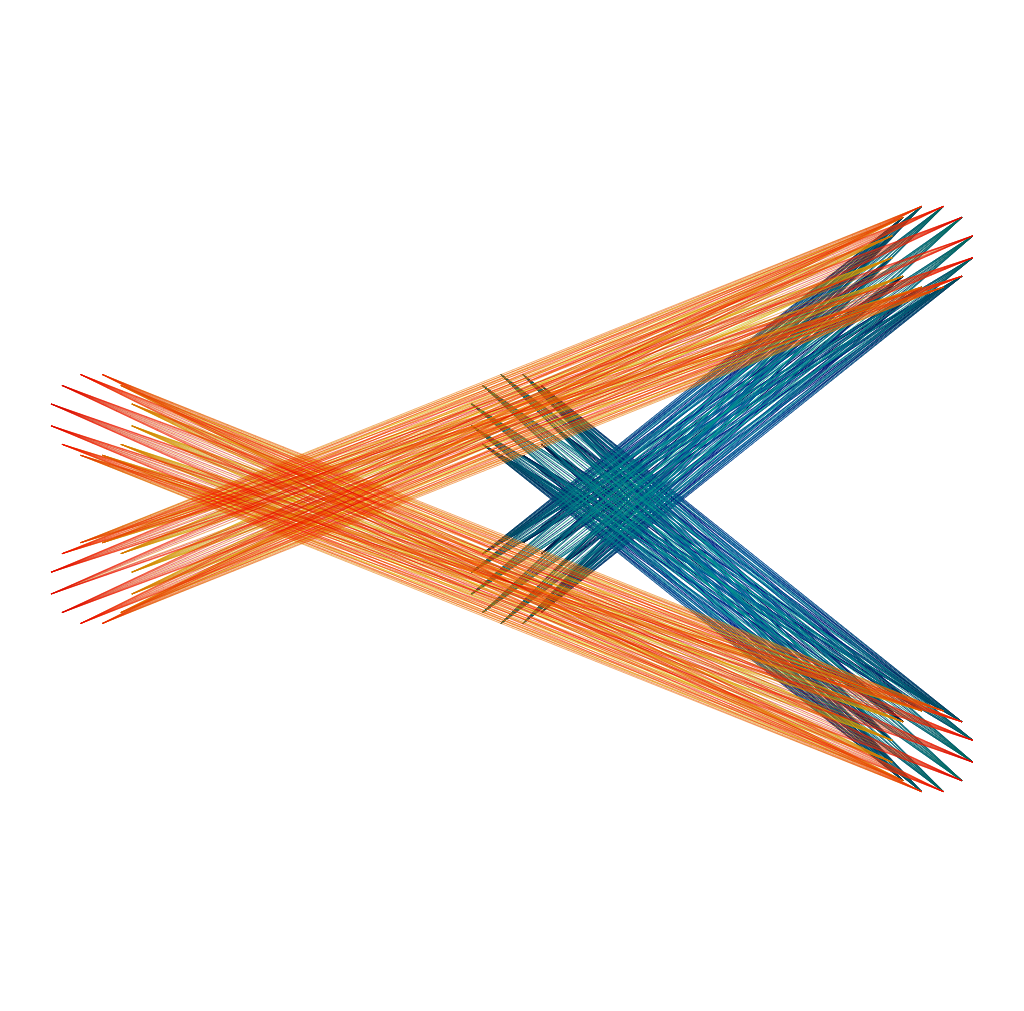
\includegraphics[width=0.48\linewidth]{metric_validation/3_straight.png}\label{fig:validation_overlap:straight}}
\subfloat[Bundled drawing]{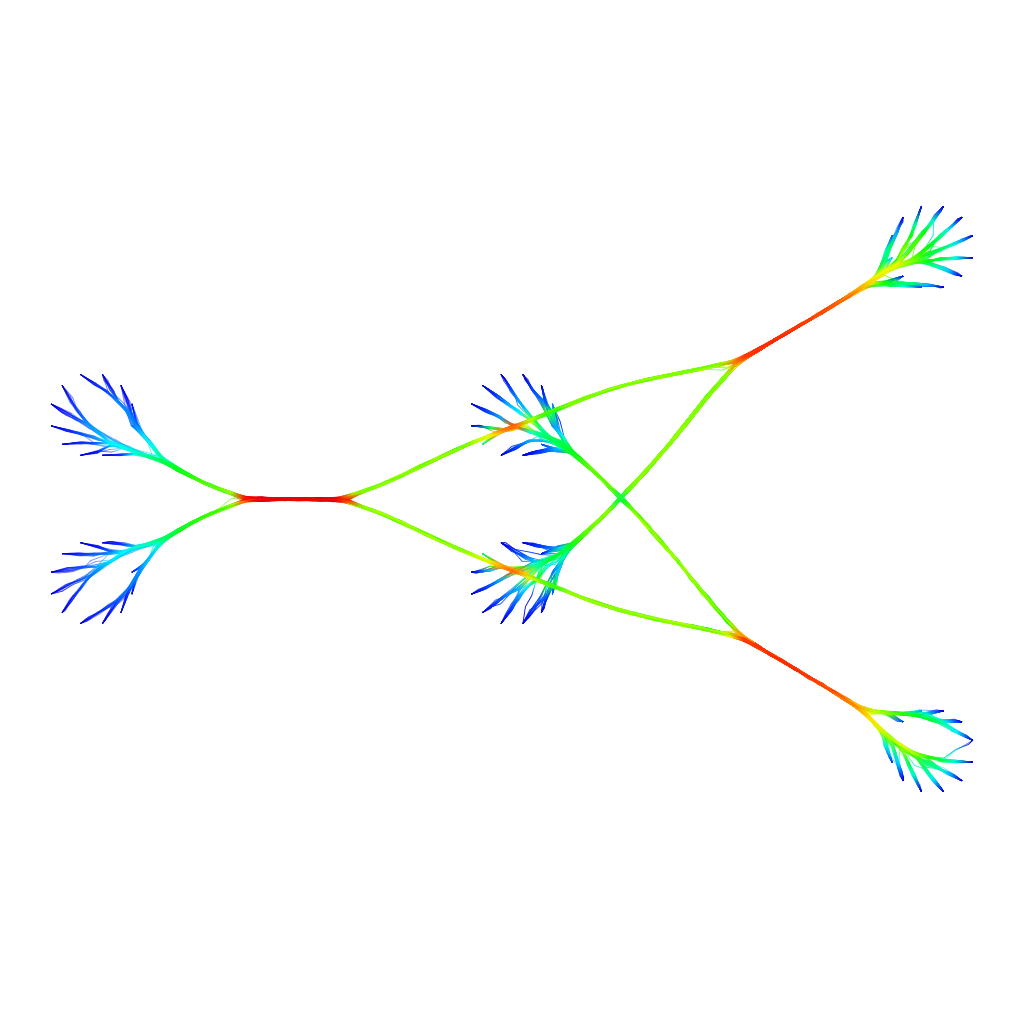
\includegraphics[width=0.48\linewidth]{metric_validation/3_bundled.png}\label{fig:validation_overlap:ambiguity}}\\
\caption{Example of $\omega$ validation with overlapping paths and endpoint clusters.}
\end{figure}

Finally, we consider a complex example with multiple ambiguous crossings and overlapping paths. Figure \ref{fig:validation_complex:straight} presents a network in the shape of a hexagon, where each cluster is connected to every other cluster. The bundled visualization (Figure \ref{fig:validation_complex:ambiguity}) creates a complex network of bundles, with multiple ambiguous crossings and overlapping paths. $\omega$ effectively captures this complexity, as shown in Figure \ref{fig:validation_complex:ambiguity}. Tracing bundles from each cluster, it is possible to see that every time divergent bundles meet, \textit{i.e.} where there is loss of perceived connectivity, $\omega$ assigns high ambiguity values to the region. The highlighted regions present examples of such ambiguous regions.

\begin{figure}[ht]
\centering
\subfloat[Input drawing]{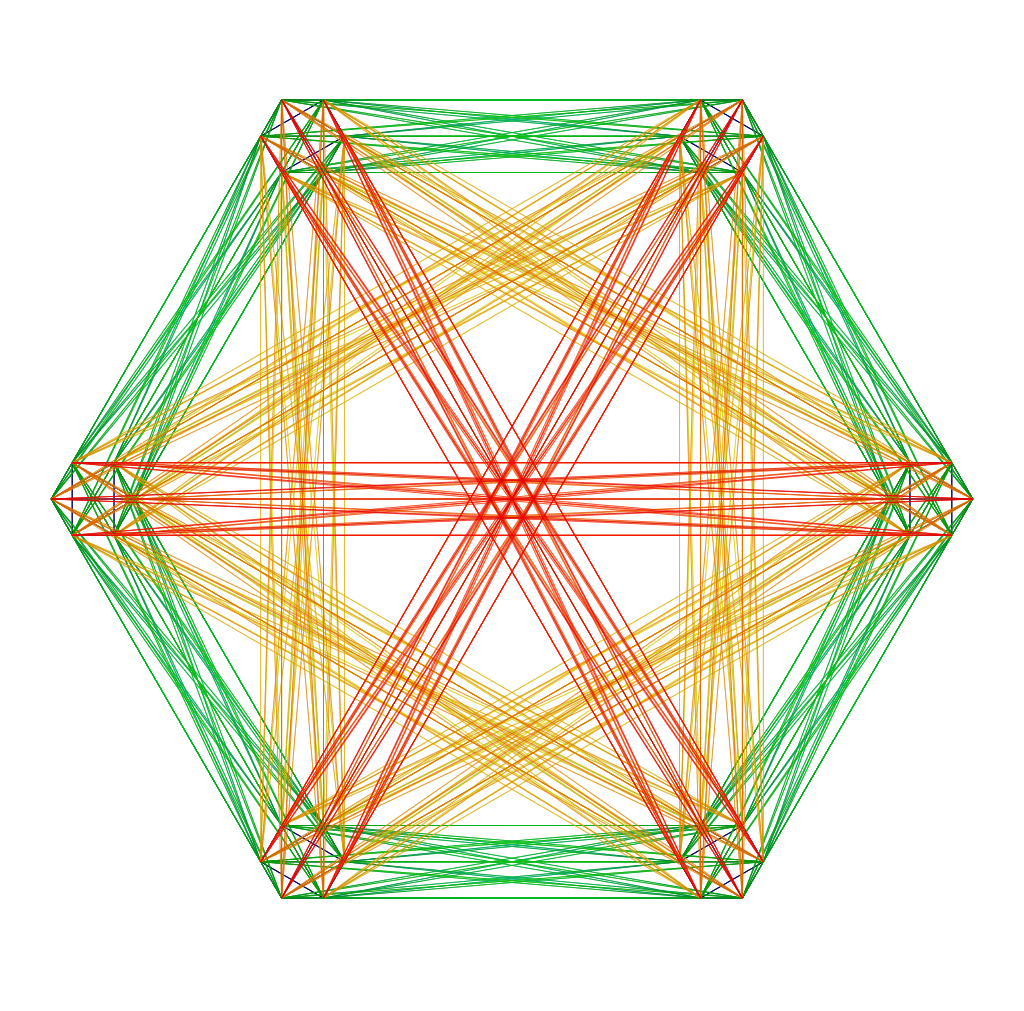
\includegraphics[width=0.48\linewidth]{metric_validation/4_straight.png}\label{fig:validation_complex:straight}}
\subfloat[Bundled drawing]{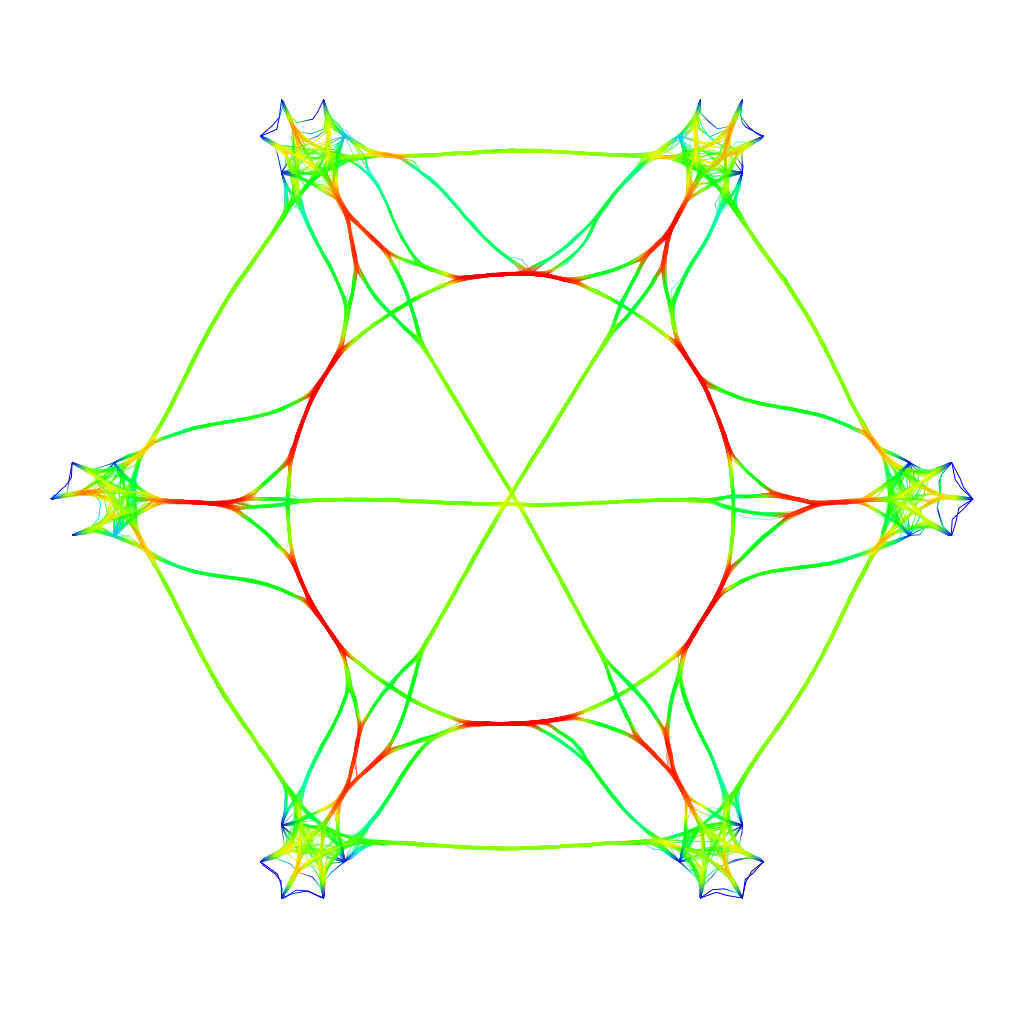
\includegraphics[width=0.48\linewidth]{metric_validation/4_bundled.png}\label{fig:validation_complex:ambiguity}}\\
\caption{Example of $\omega$ validation with complex data.}
\end{figure}


These validation cases demonstrate that $\omega$ successfully captures ambiguity patterns across a spectrum of complexity, from simple crossings to intricate bundling scenarios. The metric consistently identifies regions where connectivity information is compromised while appropriately handling cases where visual complexity does not necessarily imply ambiguity, such as bundle-cluster overlaps. Through these test cases, we have shown that $\omega$ fulfills its design goals: providing localized ambiguity measurements and accounting for path similarity in crossing regions. This validation establishes $\omega$ as a reliable tool for evaluating and potentially improving bundled graph visualizations.

% ------- SUBSECTION -------

\subsection{Parameters}

Our ambiguity metric presents three distinct parameters to customize the view of the user:

\begin{itemize}
\item $r \in \mathbb{N}$: This is the radius of neighborhood $N_r$ in step 1, and the radius of the convolution kernel in step 3. Lower values reduce the area of influence of ambiguous crossings, increasing the sharpness of the ambiguity map. Meanwhile, higher values increase the spread of ambiguity to neighbouring regions and smooth out the ambiguity values across the map. Typical values for $r$ range from 3 to 7. Figure \ref{fig:param_r} compares different values of $r$ with other parameters fixed.

\begin{figure}[ht]
\centering
\subfloat[$r = 3$]{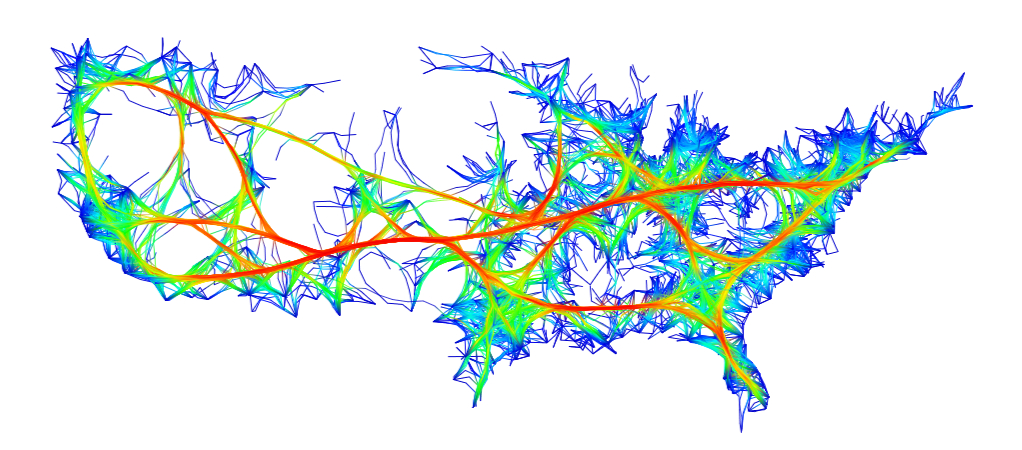
\includegraphics[width=0.48\linewidth]{params/r_3.png}}
\subfloat[$r = 5$]{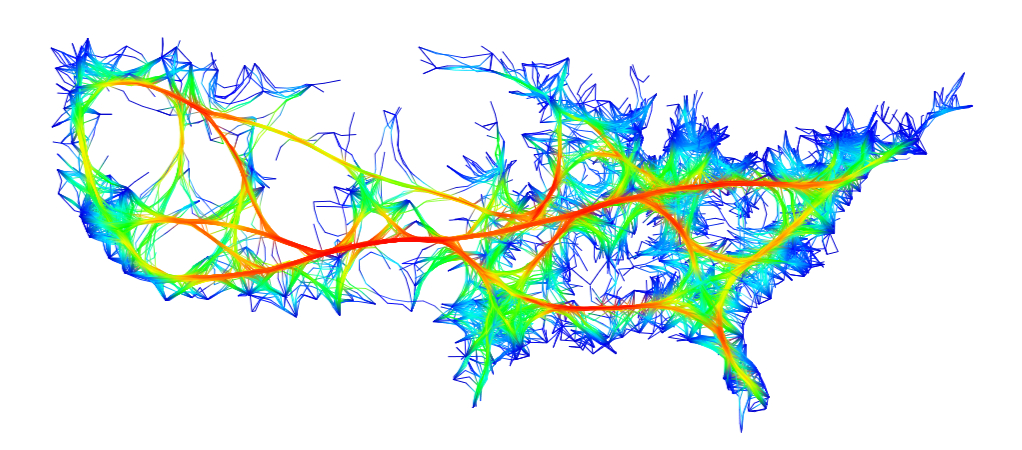
\includegraphics[width=0.48\linewidth]{params/r_5.png}}\\
\subfloat[$r = 7$]{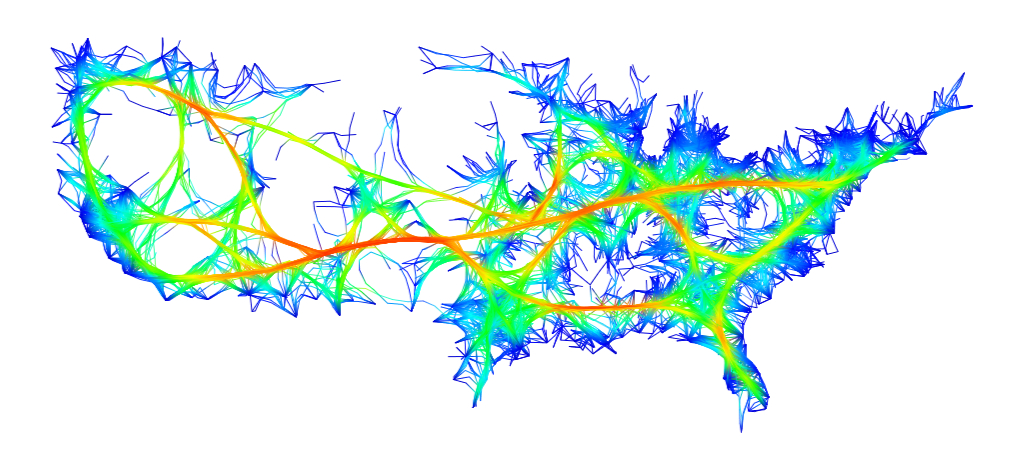
\includegraphics[width=0.48\linewidth]{params/r_7.png}}
\subfloat[$r = 9$]{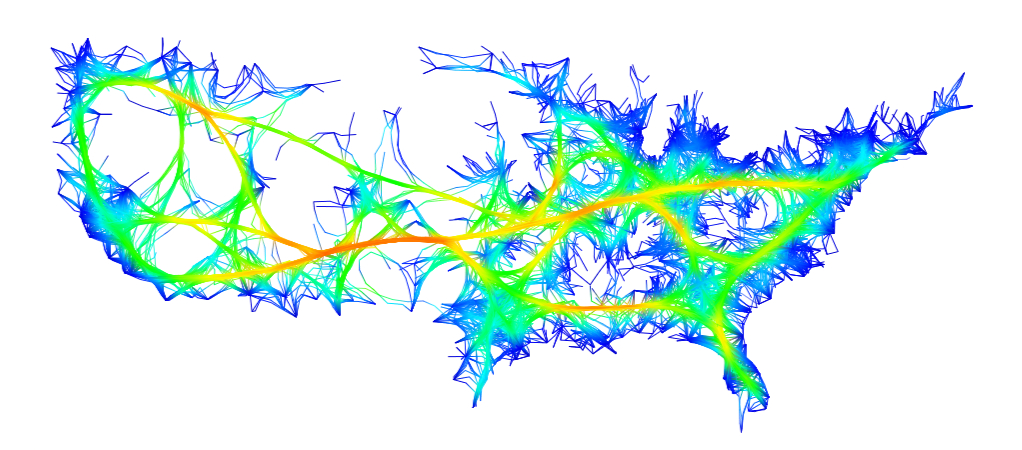
\includegraphics[width=0.48\linewidth]{params/r_9.png}}\\
\caption{Comparison of the same drawing with varying $r$ and all other parameters fixed.}
\label{fig:param_r}
\end{figure}

\item $m \in [0, 0.5]$: This controls the modulation of ambiguity values of paths according to their distance from path endpoints, described in-depth in step 2. Lower values decrease the distance to which values are modulated, while higher values increase it. A $m$ value of 0.25 provides a good middle ground for the general case. Figure \ref{fig:param_m} compares different values of $m$ with other parameters fixed.

\begin{figure}[ht]
\centering
\subfloat[$m = 0$]{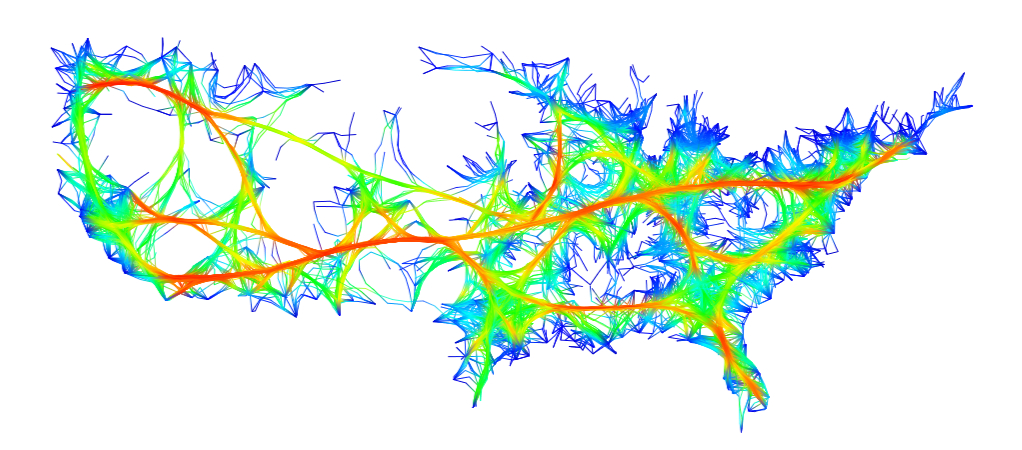
\includegraphics[width=0.48\linewidth]{params/m_.00.png}}
\subfloat[$m = 0.25$]{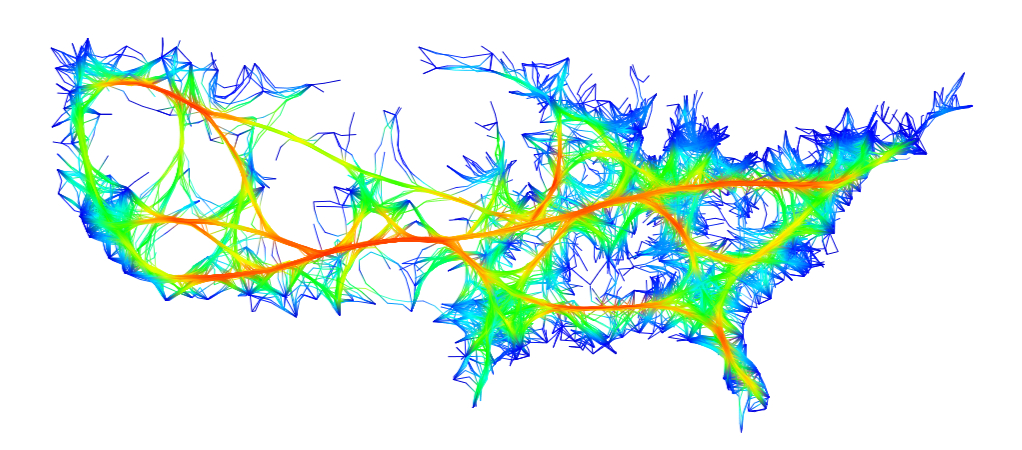
\includegraphics[width=0.48\linewidth]{params/m_.25.png}}\\
\subfloat[$m = 0.50$]{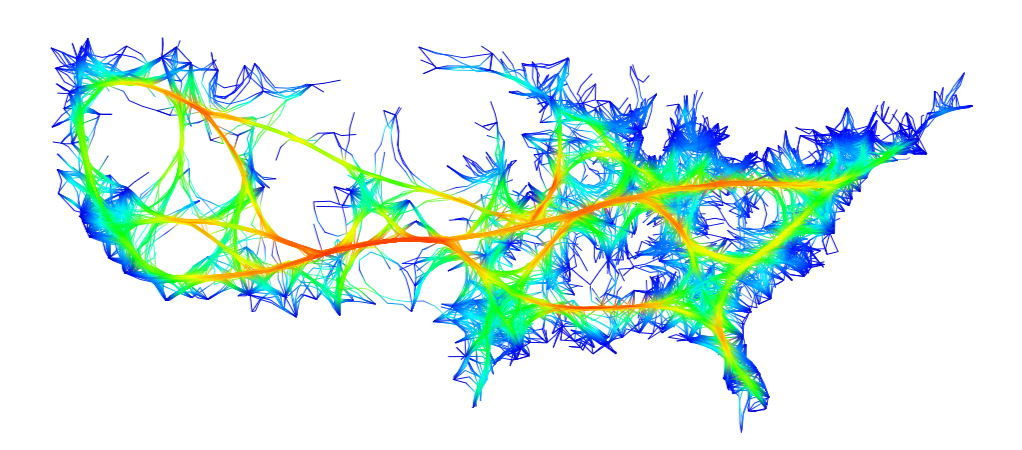
\includegraphics[width=0.48\linewidth]{params/m_.50.png}}
\subfloat[$m = 0.75$]{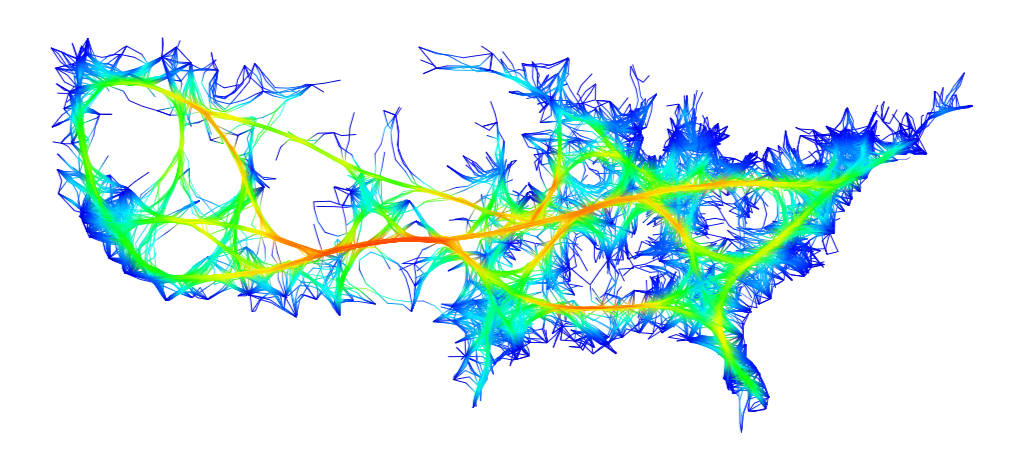
\includegraphics[width=0.48\linewidth]{params/m_.75.png}}\\
\caption{Comparison of the same drawing with varying $m$ and all other parameters fixed.}
\label{fig:param_m}
\end{figure}

\item $c \in \mathbb{R}_{+}$: This defines the threshold used to normalize the ambiguity values across the map, as described in step 4. Lower values will be more sensitive to ambiguity, presenting higher final values from lower raw ambiguity values. The opposite holds for higher values of $c$. As we adjust $c$ according $r$, a good all-round value for $c$ is 1. Figure \ref{fig:param_m} compares different values of $c$ with other parameters fixed.

\begin{figure}[ht]
\centering
\subfloat[$c = 0.6$]{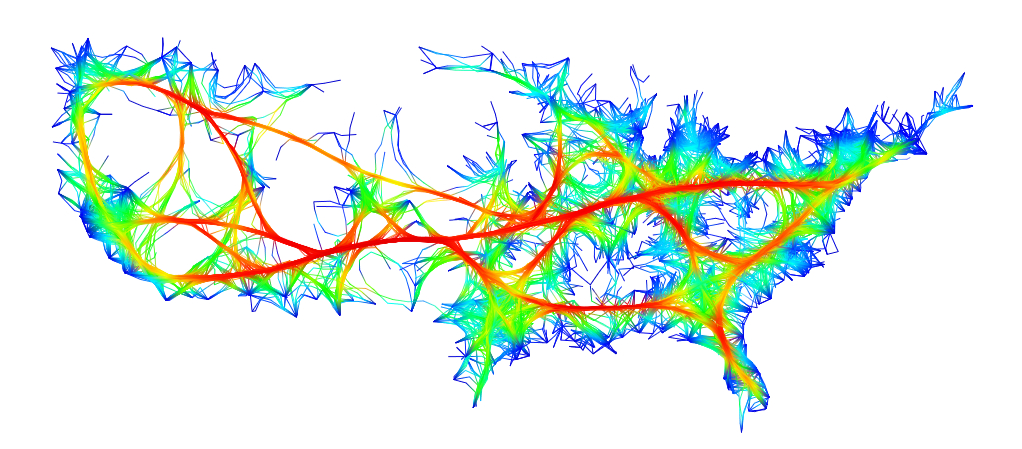
\includegraphics[width=0.48\linewidth]{params/c_0.6.png}}
\subfloat[$c = 0.8$]{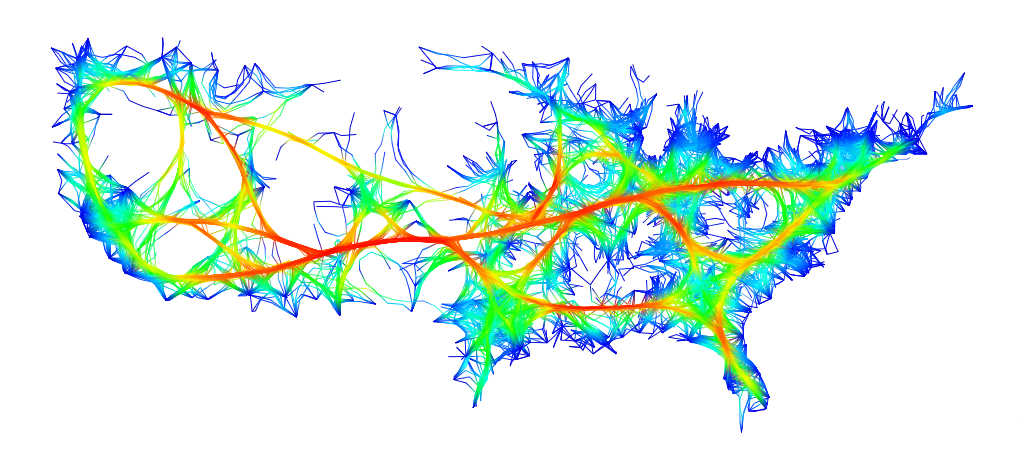
\includegraphics[width=0.48\linewidth]{params/c_0.8.png}}\\
\subfloat[$c = 1.0$]{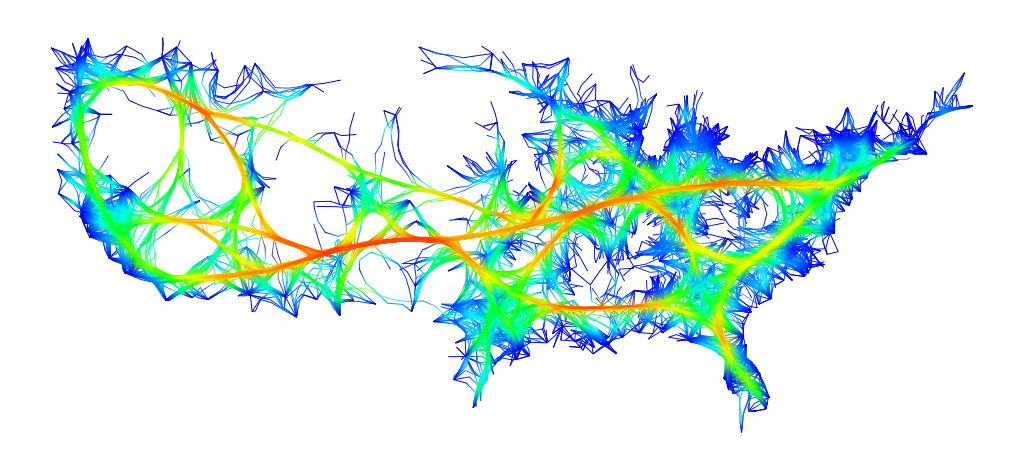
\includegraphics[width=0.48\linewidth]{params/c_1.0.png}}
\subfloat[$c = 1.2$]{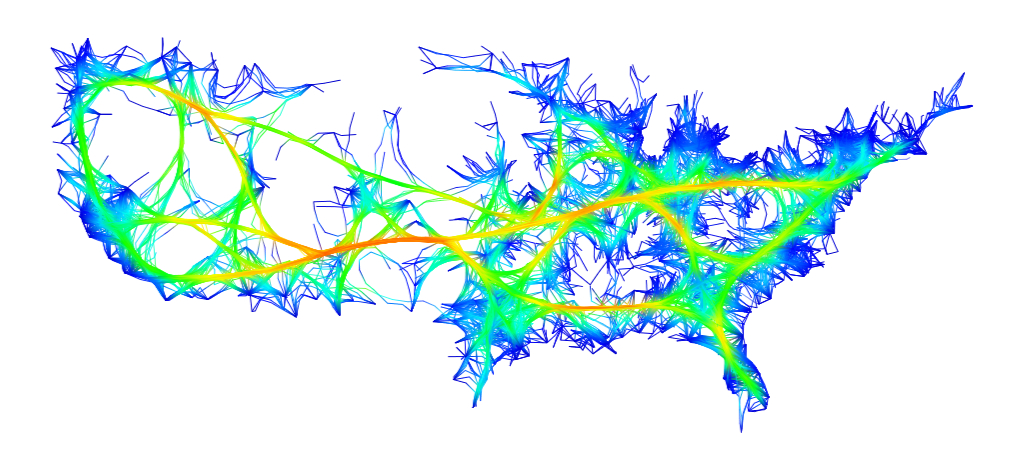
\includegraphics[width=0.48\linewidth]{params/c_1.2.png}}\\
\caption{Comparison of the same drawing with varying $m$ and all other parameters fixed.}
\label{fig:param_m}
\end{figure}

\end{itemize}

%!TeX root=../paper.tex

\section{Ambiguity-Avoidance Bundling}\label{sec:bundling}

With the ambiguity metric defined, we now introduce our method for reducing ambiguity in graph bundling. A key advantage of our approach is its modularity; rather than developing a standalone bundling algorithm, we propose a framework that can be integrated with existing techniques. This allows us to leverage the strengths of established bundling methods while adding ambiguity-avoidance to the stack. By adapting to the underlying characteristics of different bundling algorithms, our approach offers broad applicability and can be tailored to specific problem domains.

Initially, we explore two distinct implementations of this framework: a post-processing method that can be applied universally and a modification specifically designed for iterative bundling techniques, which operates by adjusting path point displacement during each iteration. Due to limitations encountered with the post-processing implementation, we restrict our analysis and evaluation to the iterative bundling modification.


\subsection{Post-processing Approach}

Our initial investigation focused on developing a post-processing solution to reduce ambiguity in bundled visualizations. This approach was particularly appealing due to its potential for universal application—it could theoretically enhance any existing bundling method without requiring modifications to the core bundling algorithm. The concept involved locally interpolating between the bundled and unbundled states based on the measured ambiguity in each region.

% lucas: should I add an image of the "unbundled" bundled visualization to "prove" that the results were indeed bad? Also, I added a flag so that I can easily enable or disable this post-processing step, should I mention it in the paper?
However, this approach quickly revealed fundamental limitations. Attempting to ``unbundle" high-ambiguity regions generated excessive visual clutter, while trying to bundle these areas again merely recreated the initial bundled state we were trying to modify. These immediate practical constraints led us to abandon the post-processing approach in favor of a more promising direction: integrating ambiguity awareness directly into the iterative bundling process.


\subsection{Image Based Ambiguity-Avoidance Bundling (IBAVB)}

After exploring ambiguity-avoidance through post-processing, we focused on developing a method that could influence bundle formation during the iterative process itself, as it would grant us more control over it. Our approach, which we call Image Based Ambiguity-Avoidance Bundling (IBAVB), operates by modifying the core mechanics of iterative bundling algorithms. These algorithms typically move paths incrementally at each iteration according to specific vector fields or transformation rules. IBAVB leverages this characteristic by using $\omega$ to influence these movement patterns, steering paths toward configurations that generate less ambiguity.

During our investigation, we explored several strategies for incorporating ambiguity awareness into the bundling process, including modulating bundling speed, implementing repulsion forces, and interpolating bundling vectors. Through both qualitative and quantitative evaluation, we found that the simplest approach, modulating bundling speed based on local ambiguity, produced the most effective results. A part of these are present as supplementary material. Next, we present the mathematical formulation of this approach, demonstrating how we integrate ambiguity awareness into the bundling process through speed modulation.

\textbf{IBAVB:} The overview idea behind IBAVB is simple, if a path is being moved to a region with less ambiguity, we do nothing; if a path is being moved to a region with more ambiguity, we slow down the deformation of the path according to the destination ambiguity. Let $S : \mathbb{R}^2 \rightarrow \mathbb{R}^2$ be the step function that $B$ uses for bundling applied to each point in paths; we want to define IBAVB for a given point $\mathbf{a} \in p_i$ with $\eta$, where $p_i \in D(P)$, in a way that $\eta$ replaces $S$ in the original bundling method. For such, we consider the vector $\mathbf{d} = S(\mathbf{a}) - \mathbf{a}$ to to define $\eta$ as follows:

\textbf{IBAVB Formulation:} The fundamental principle of IBAVB is to modulate the bundling process based on local ambiguity. When a path segment moves toward a region of lower ambiguity, the bundling proceeds normally; however, when moving toward higher ambiguity regions, we attenuate the deformation proportionally to the destination's ambiguity level. More formally, let $S : \mathbb{R}^2 \rightarrow \mathbb{R}^2$ be the step function that bundling method $B$ applies to each point in the path set. We define IBAVB's transformation function $\eta$ to replace $S$ in the original bundling method. For a given point $\mathbf{a} \in p_i$, where $p_i \in D(P)$, and displacement vector $\mathbf{d} = S(\mathbf{a}) - \mathbf{a}$, we formulate $\eta$ as follows:

\begin{align}
\mu(\mathbf{a} \in p_i) &=
\begin{cases}
    1                             & \mbox{if } \omega(S(\mathbf{a})) \leq \omega(\mathbf{a}) \\
    (1 - \omega(S(\mathbf{a})))^2 & \mbox{otherwise}
\end{cases} \\
\eta(\mathbf{a} \in p_i) &= \mu(\mathbf{a})\mathbf{d} + \mathbf{a}
\end{align}
 
With this definition, $\eta$ uses both the original and displaced points to control the bundling speed of $S$ for all $\mathbf{a} \in p_i$, $p_i \in D(P)$. This mechanism slows down bundling in regions of high ambiguity, allowing bundles to form in ways that preserve visual clarity. In the following section we demonstrate IBAVB's effectiveness through comparative examples with state-of-the-art bundling techniques.

%!TeX root=../paper.tex

\section{Experiments}\label{sec:experiments}

\clearpage

\begin{figure}[ht]
\centering
\subfloat[IBAVB 40its]{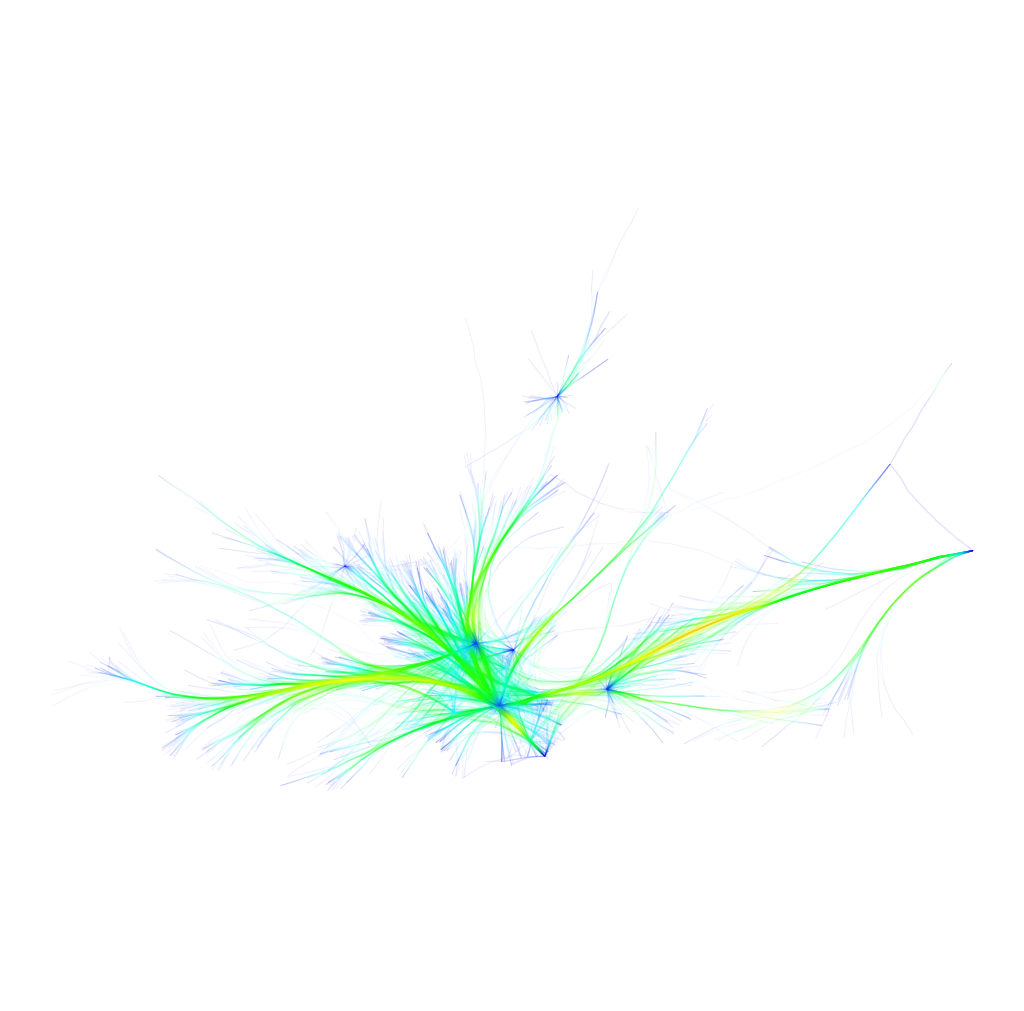
\includegraphics[width=0.48\linewidth]{rjmr-cancer/ibavb-40its-0.5eps-ambiguity-0.05alpha.png}}
\subfloat[IBAVB 40its]{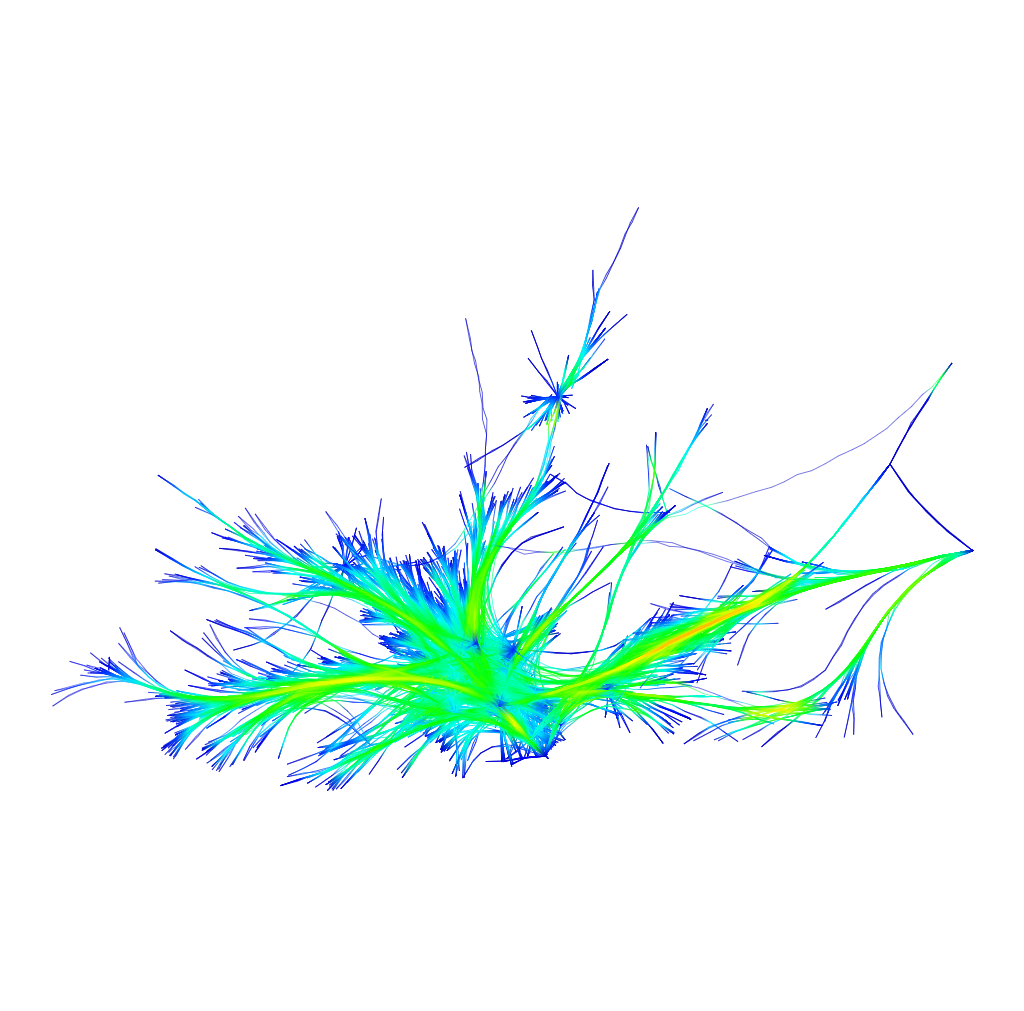
\includegraphics[width=0.48\linewidth]{rjmr-cancer/ibavb-40its-0.5eps-ambiguity.png}}\\
\subfloat[IBAVB 40its]{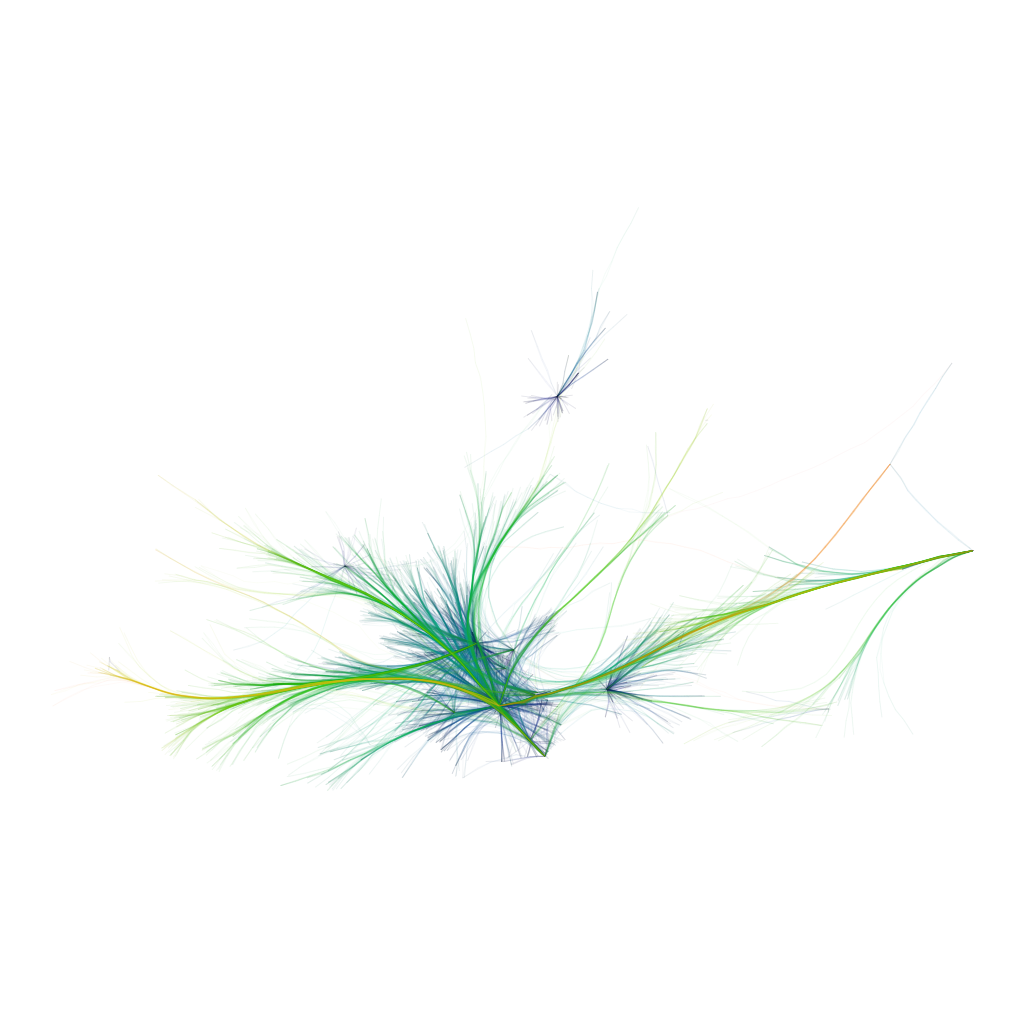
\includegraphics[width=0.48\linewidth]{rjmr-cancer/ibavb-40its-0.5eps-edgelength-0.05alpha.png}}
\subfloat[IBAVB 40its]{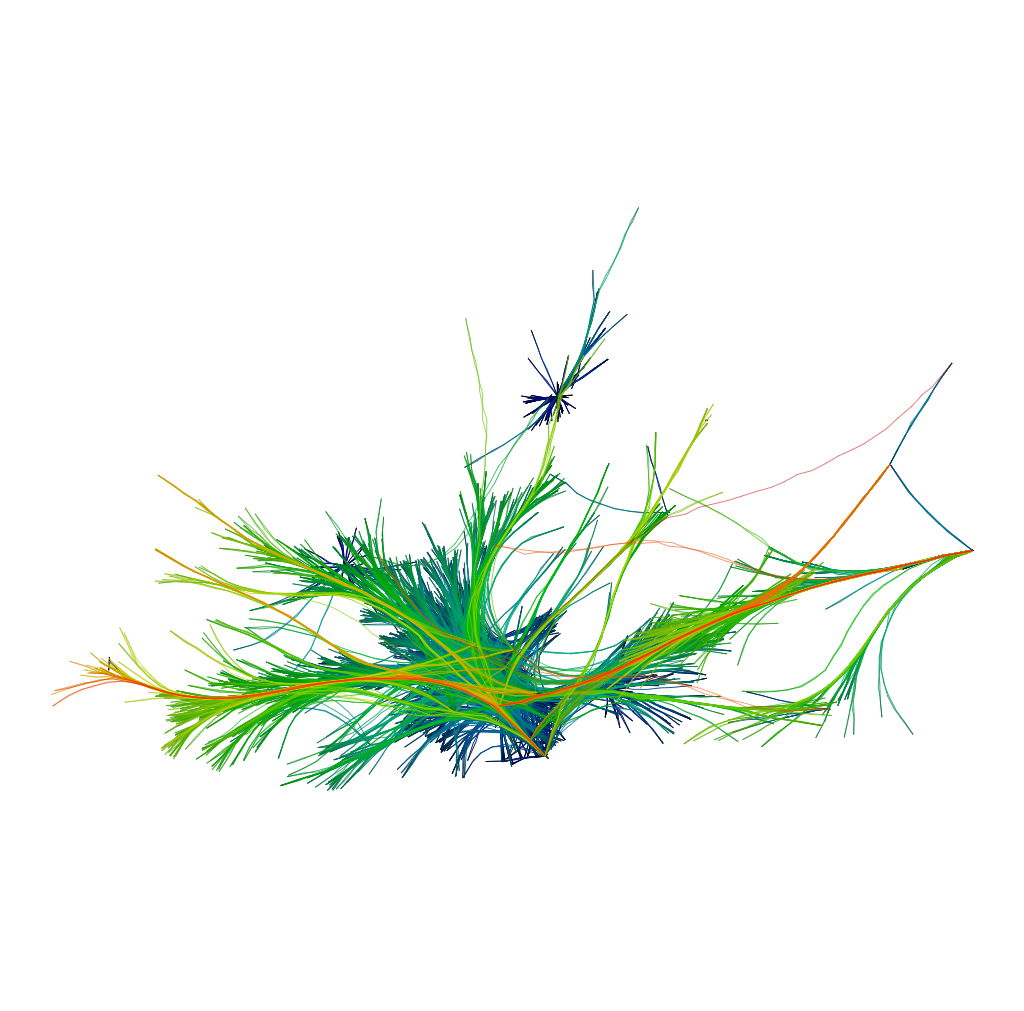
\includegraphics[width=0.48\linewidth]{rjmr-cancer/ibavb-40its-0.5eps-edgelength.png}}\\
\subfloat[IBAVB 40its]{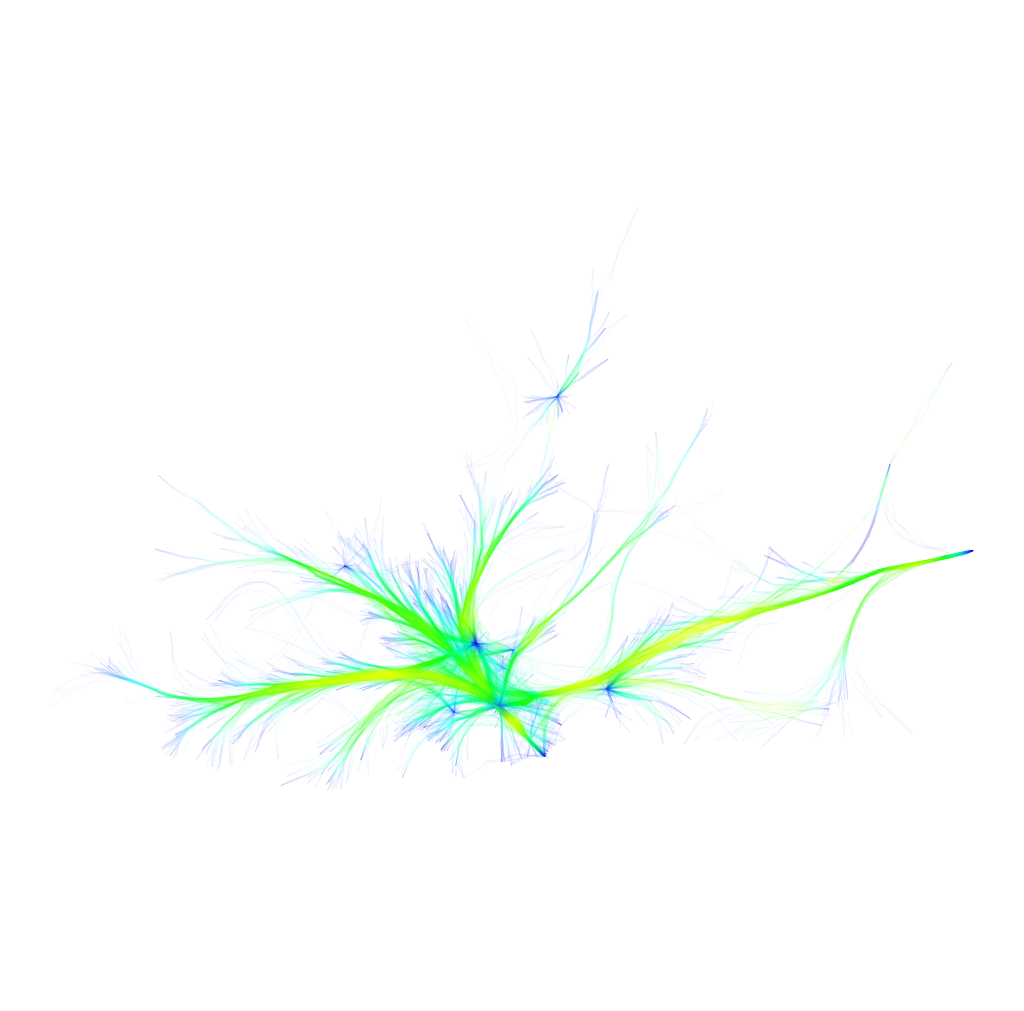
\includegraphics[width=0.48\linewidth]{rjmr-cancer/ibavb-40its-1.0eps-ambiguity-0.05alpha.png}}
\subfloat[IBAVB 40its]{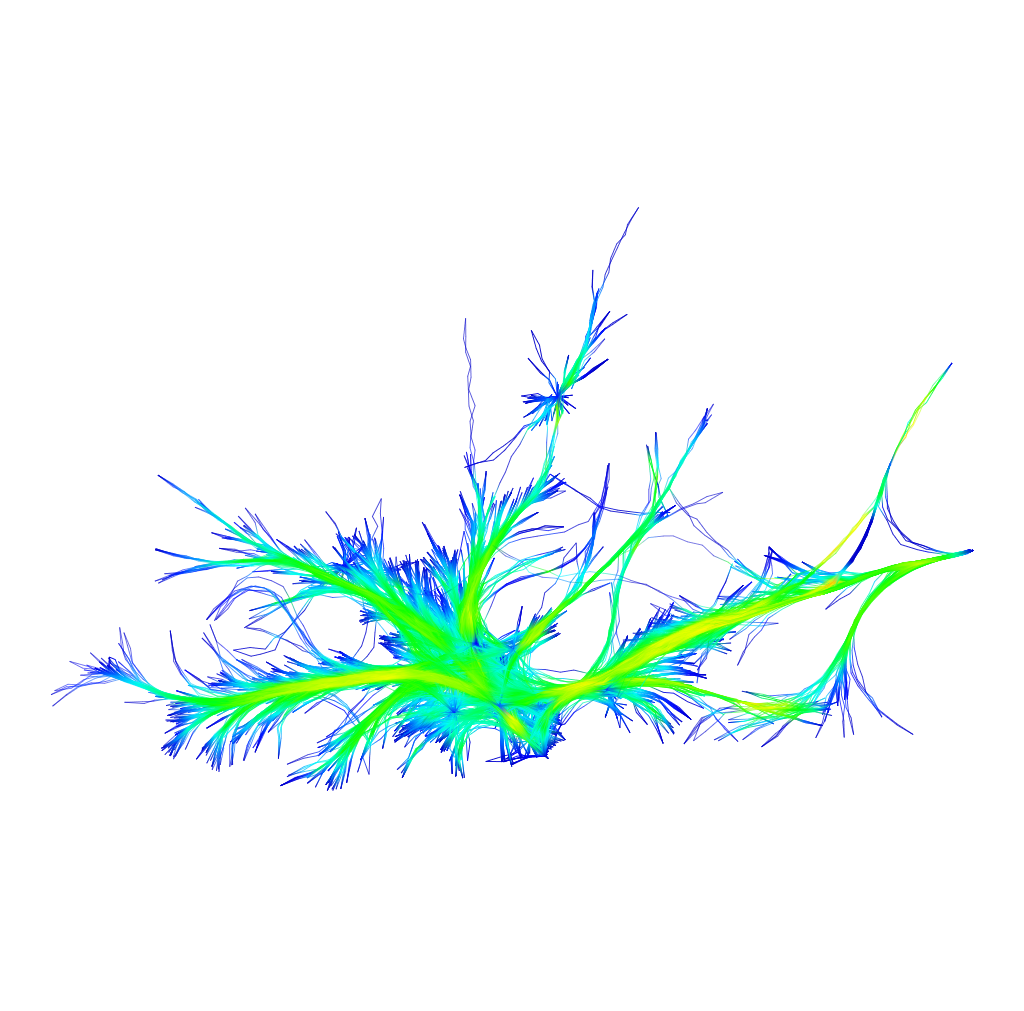
\includegraphics[width=0.48\linewidth]{rjmr-cancer/ibavb-40its-1.0eps-ambiguity.png}}\\
\subfloat[IBAVB 40its]{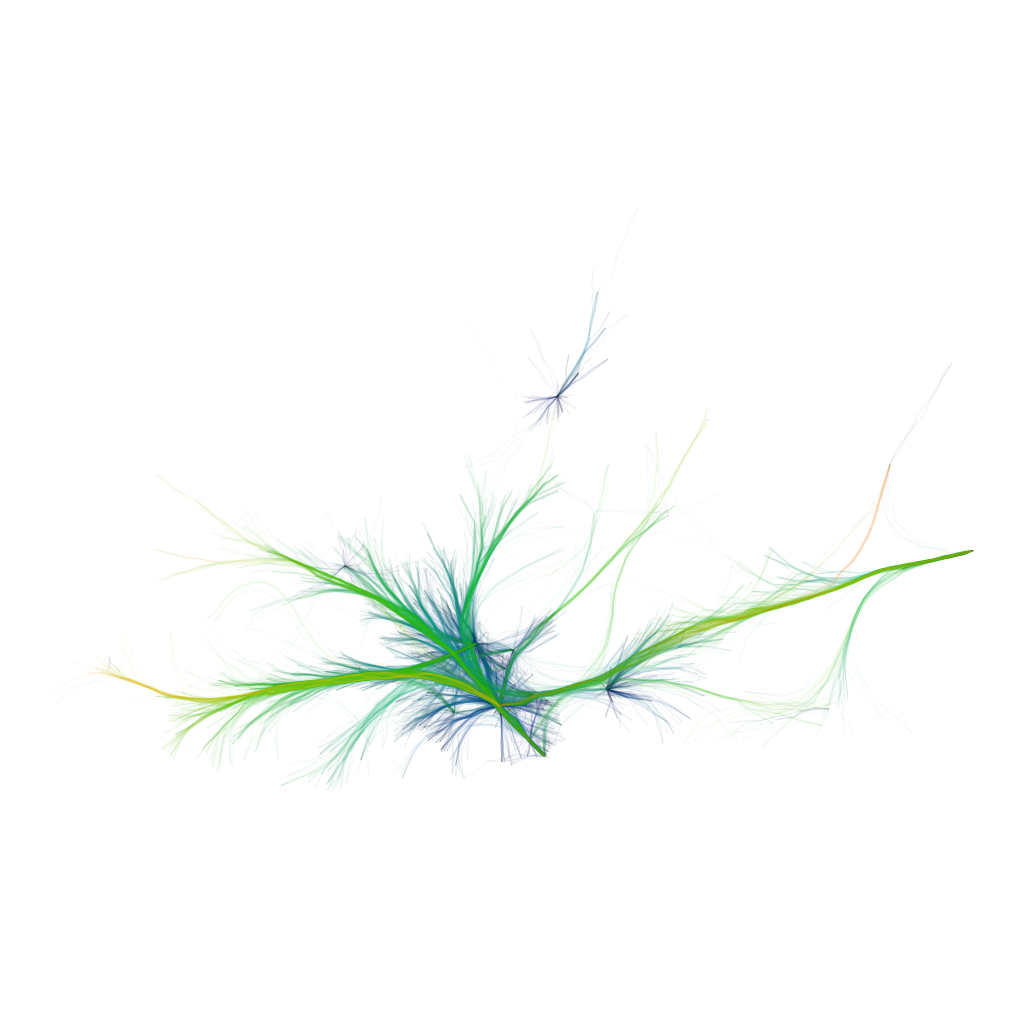
\includegraphics[width=0.48\linewidth]{rjmr-cancer/ibavb-40its-1.0eps-edgelength-0.05alpha.png}}
\subfloat[IBAVB 40its]{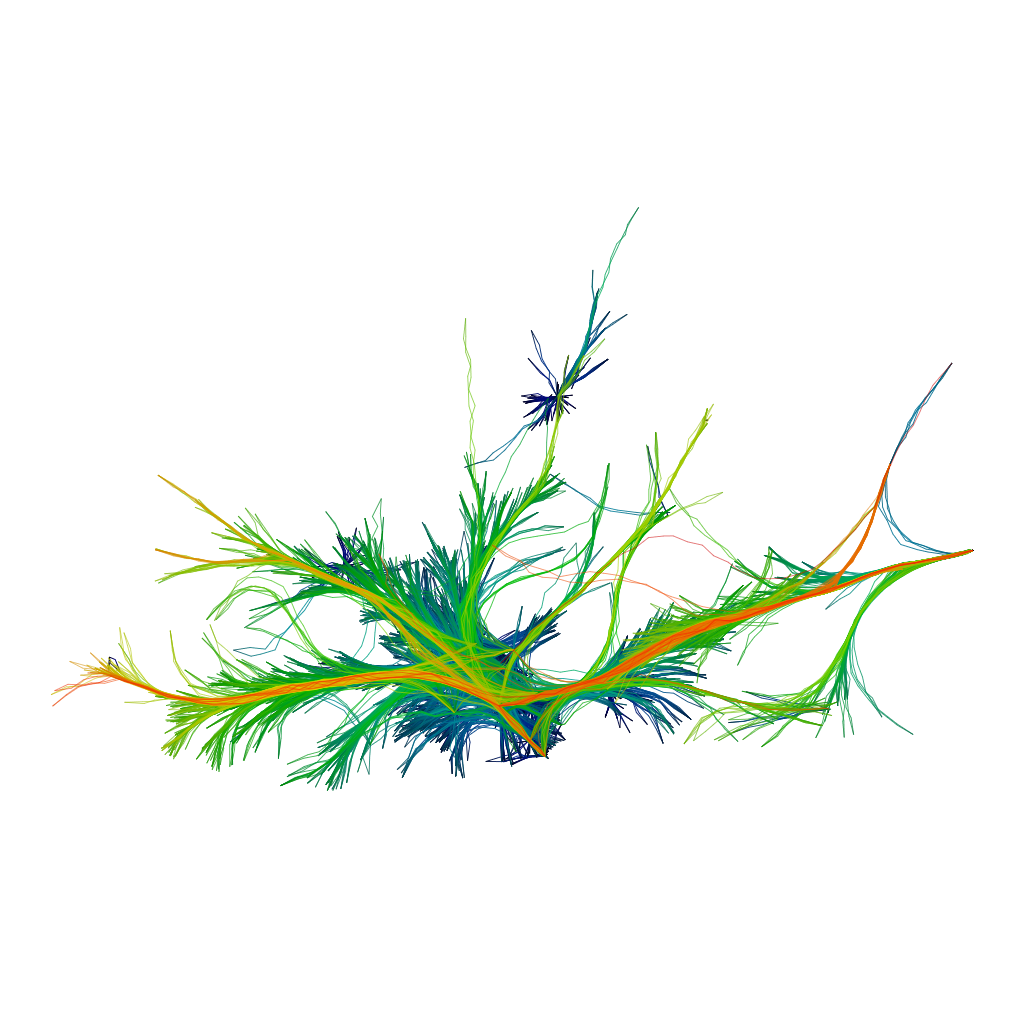
\includegraphics[width=0.48\linewidth]{rjmr-cancer/ibavb-40its-1.0eps-edgelength.png}}\\
\caption{Rio de Janeiro Metropolitan Region: breast cancer 2019/2020}
\end{figure}

\begin{figure}[ht]
\centering
\subfloat[CUBu]{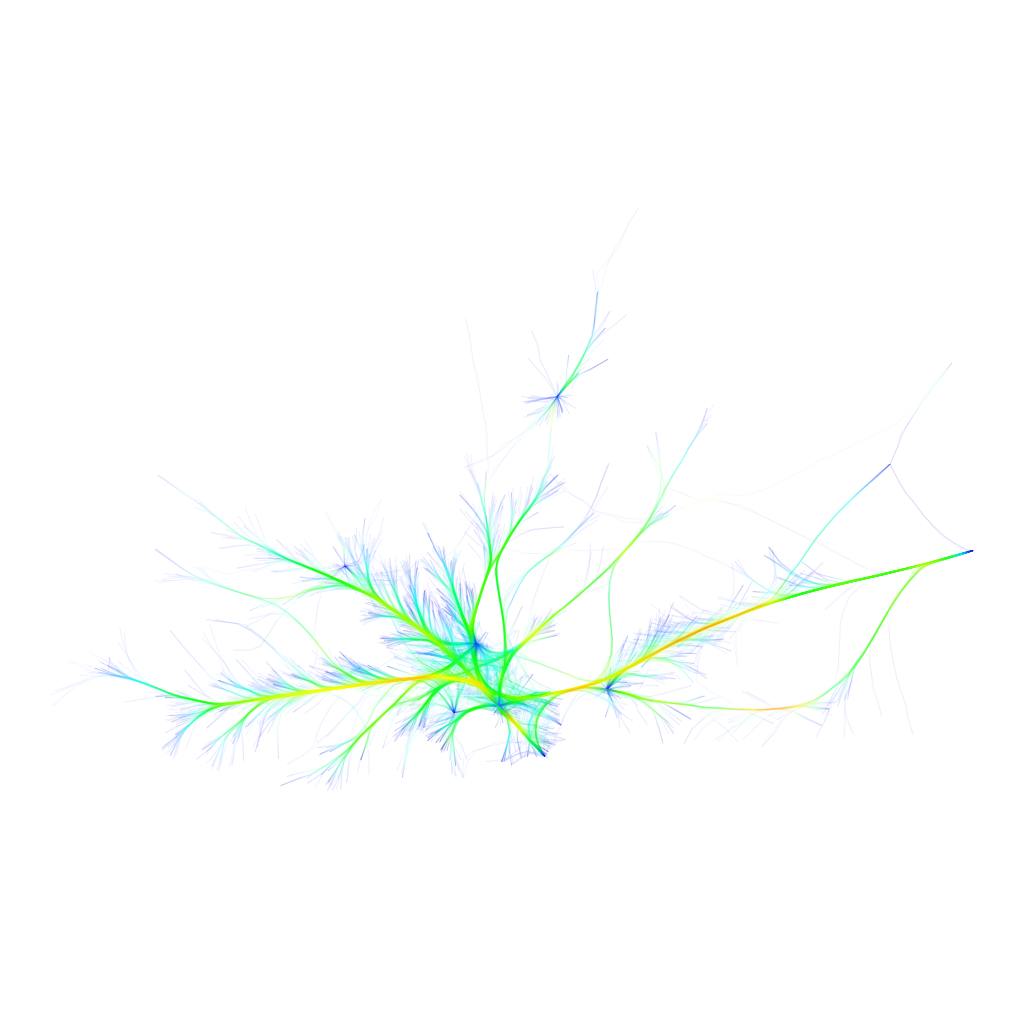
\includegraphics[width=0.48\linewidth]{rjmr-cancer/cubu-20its-ambiguity-0.05alpha.png}}
\subfloat[CUBu]{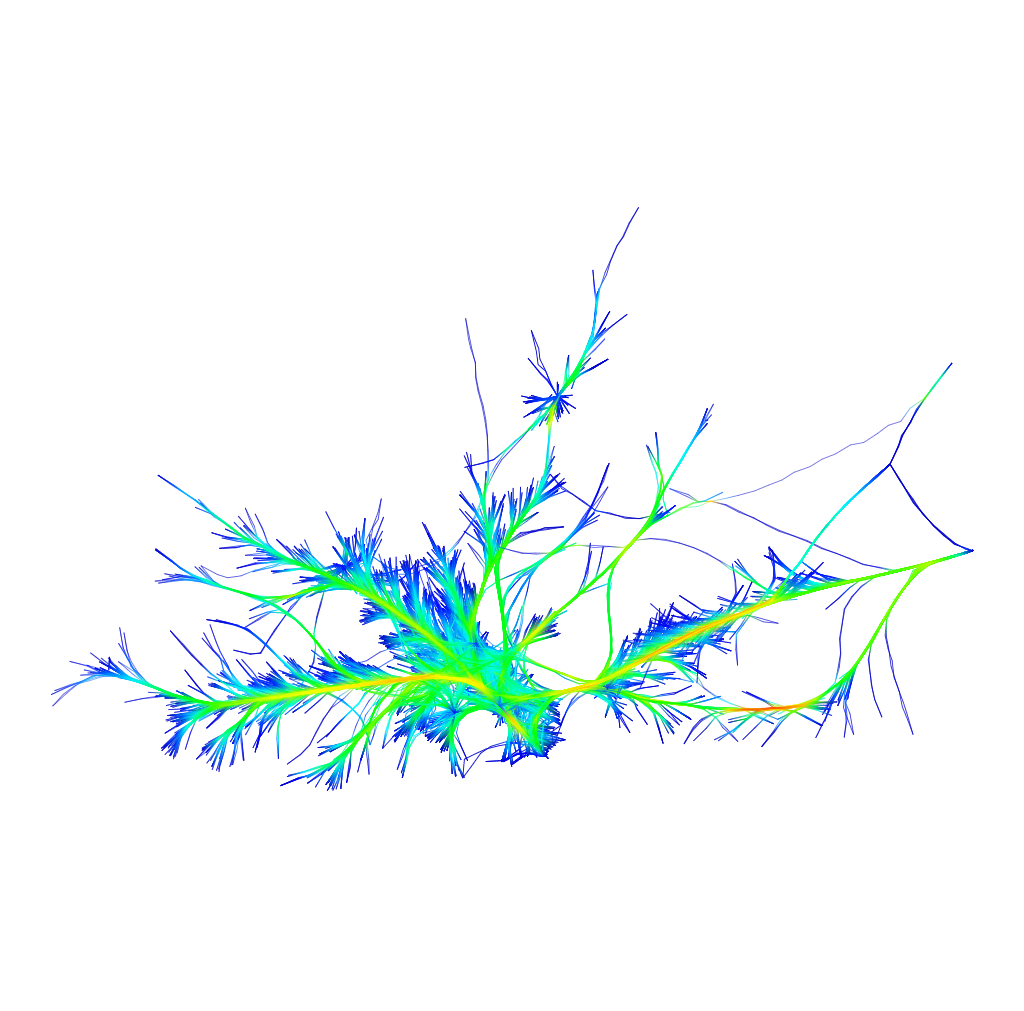
\includegraphics[width=0.48\linewidth]{rjmr-cancer/cubu-20its-ambiguity.png}}\\
\subfloat[CUBu]{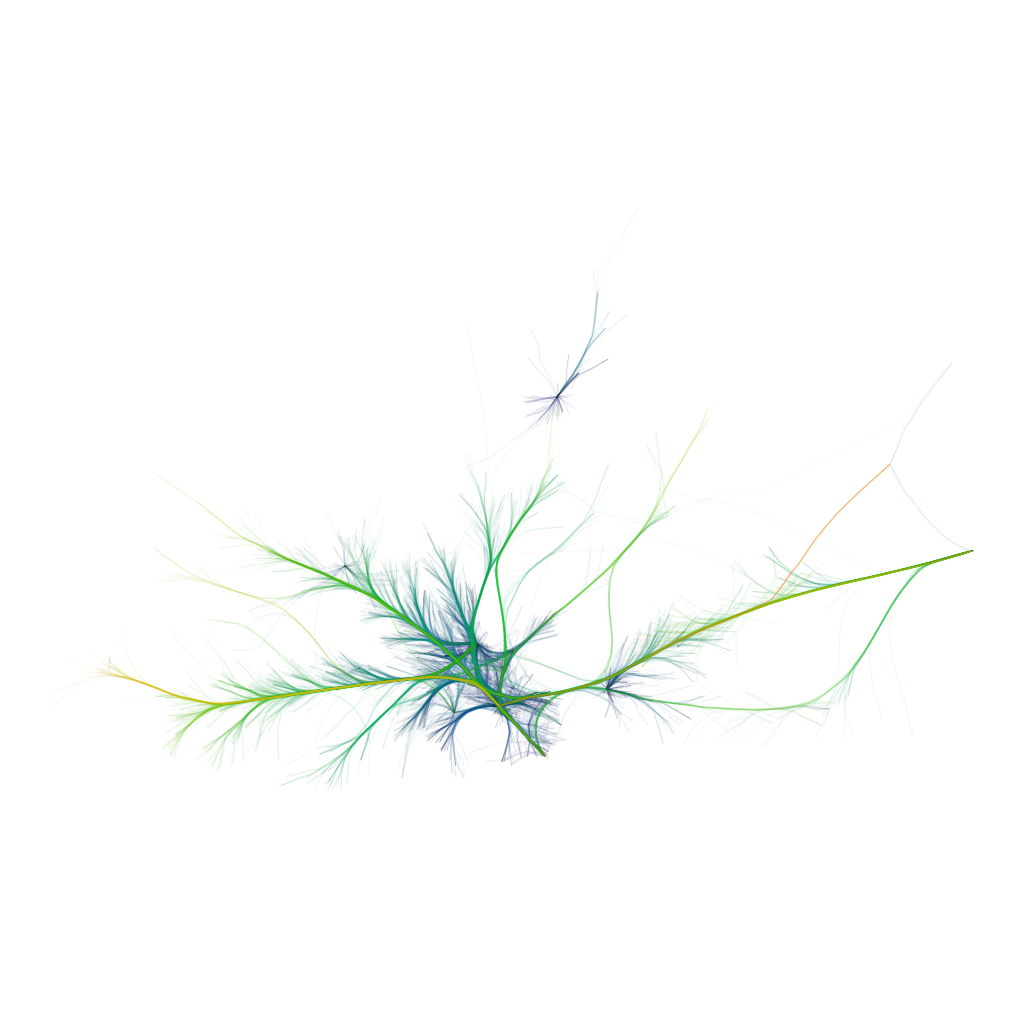
\includegraphics[width=0.48\linewidth]{rjmr-cancer/cubu-20its-edgelength-0.05alpha.png}}
\subfloat[CUBu]{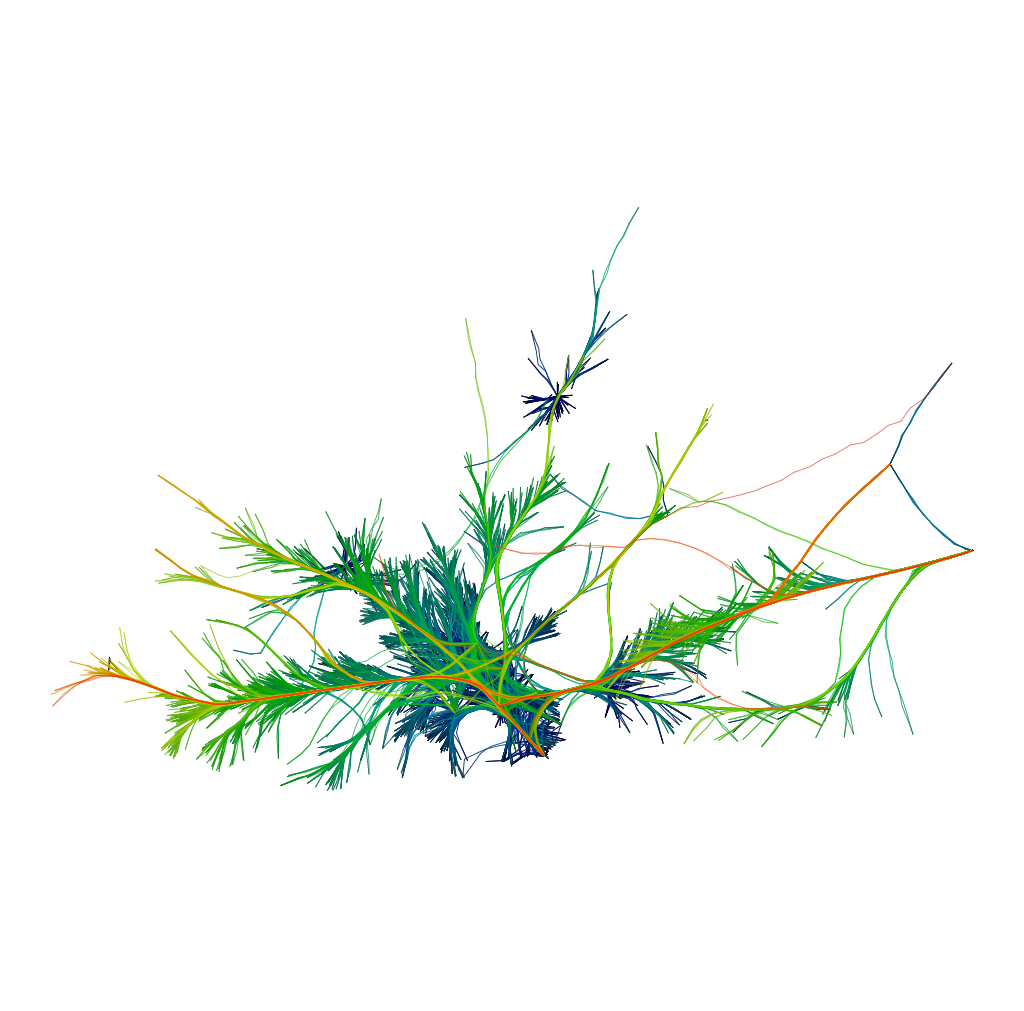
\includegraphics[width=0.48\linewidth]{rjmr-cancer/cubu-20its-edgelength.png}}\\
\caption{Rio de Janeiro Metropolitan Region: breast cancer 2019/2020}
\end{figure}

\begin{figure}[ht]
\centering
\subfloat[IBAVB 20its]{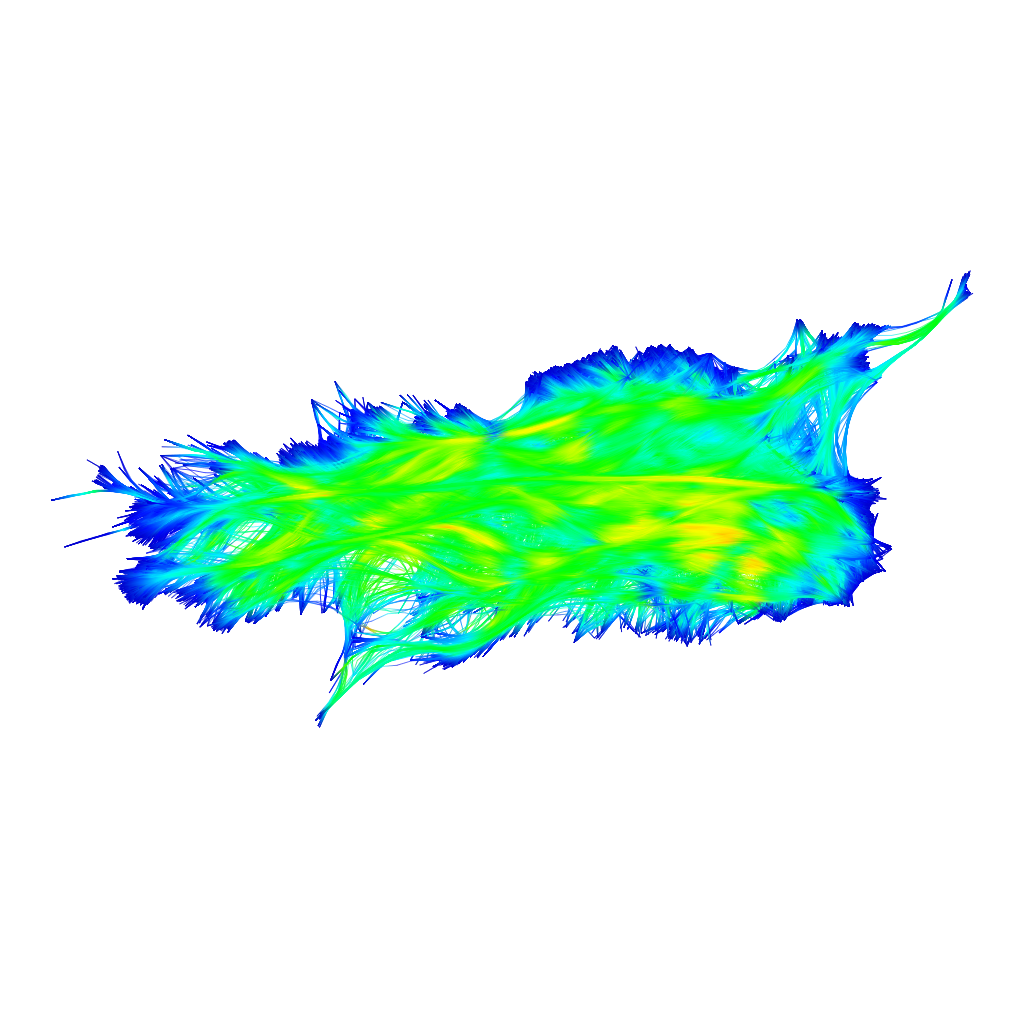
\includegraphics[width=0.48\linewidth]{rjmr-allicds/city-ibavb-20its-0.5eps-ambiguity.png}}
\subfloat[IBAVB 20its]{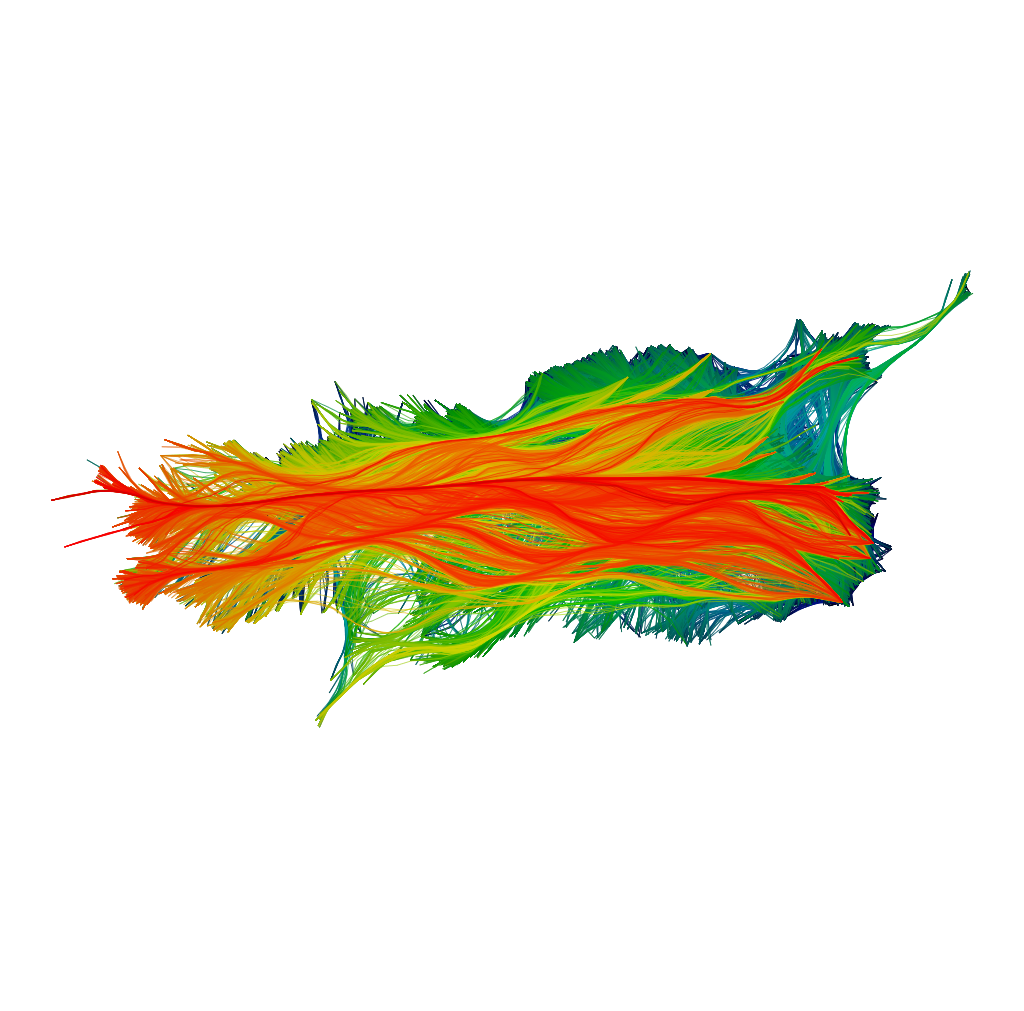
\includegraphics[width=0.48\linewidth]{rjmr-allicds/city-ibavb-20its-0.5eps-edgelength.png}} \\ 
\subfloat[IBAVB 40its]{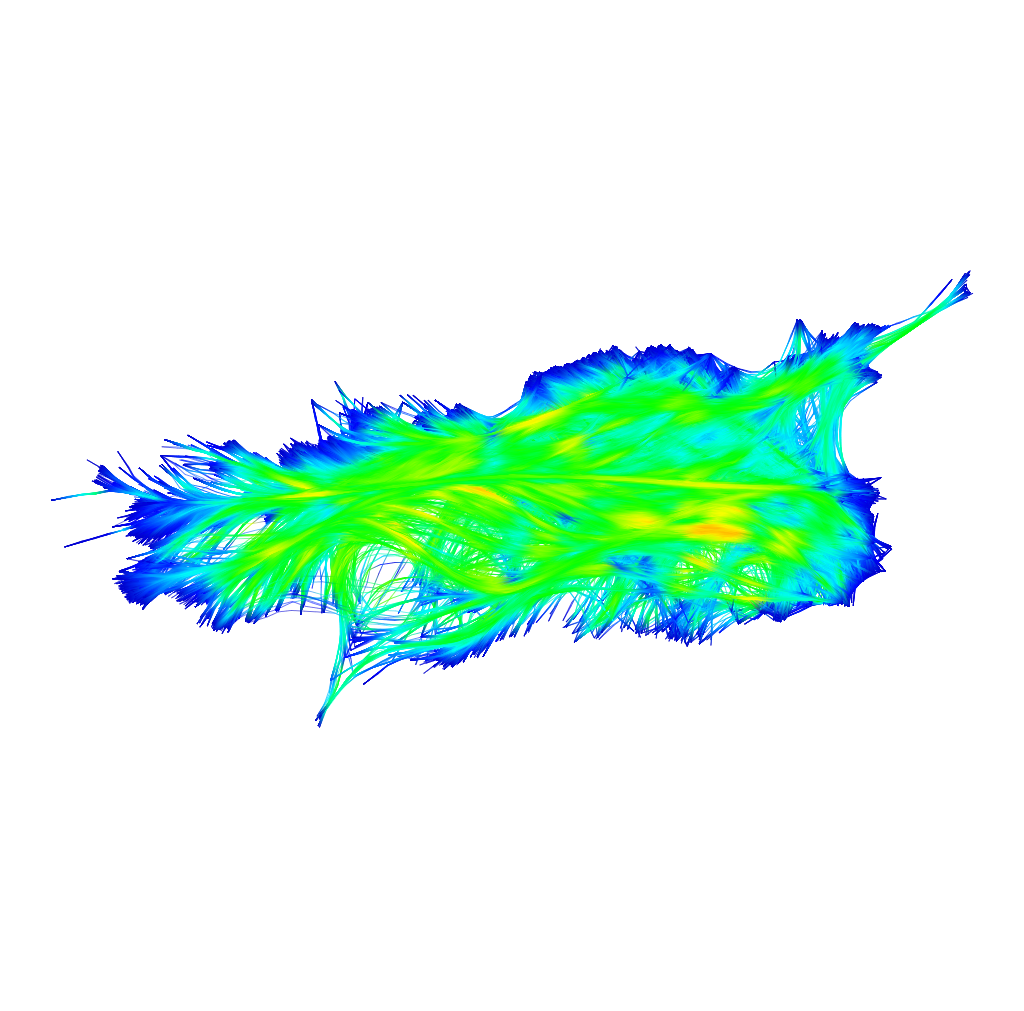
\includegraphics[width=0.48\linewidth]{rjmr-allicds/city-ibavb-40its-0.5eps-ambiguity.png}}
\subfloat[IBAVB 40its]{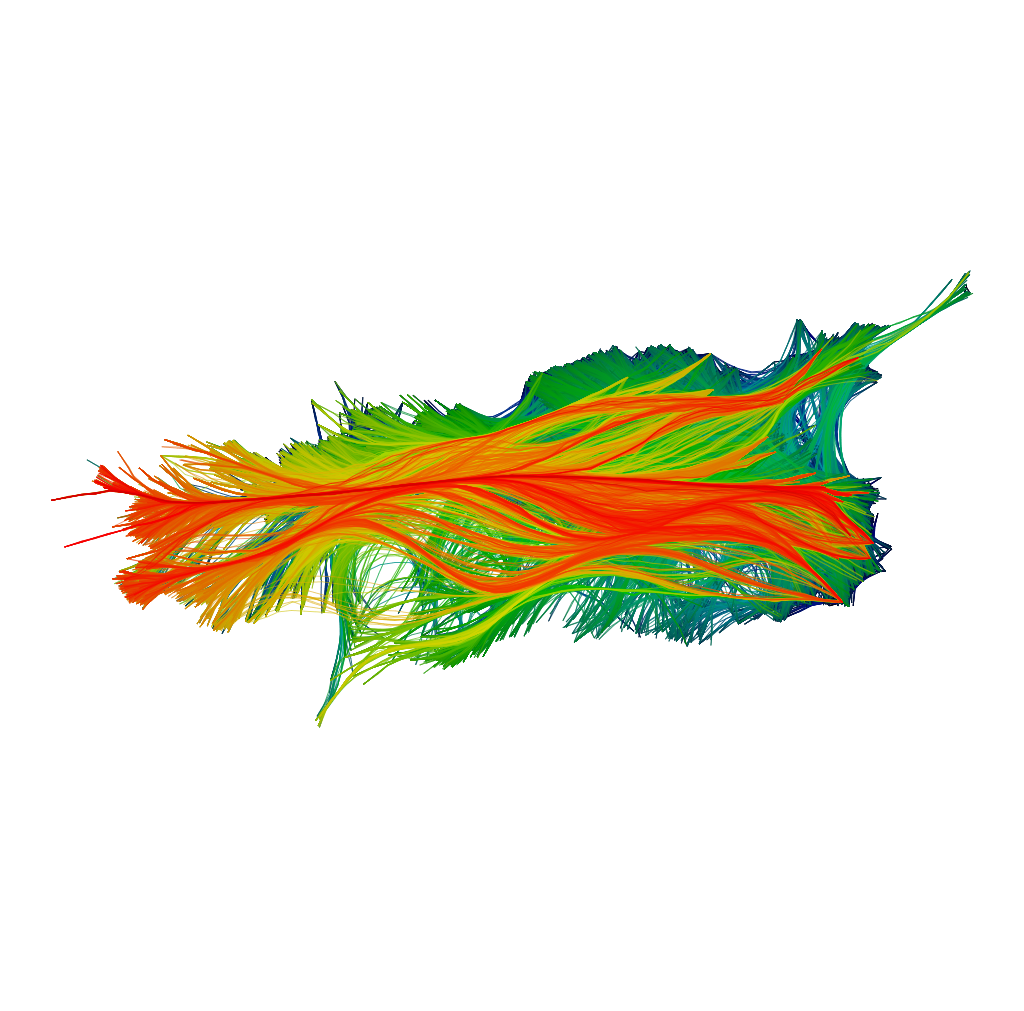
\includegraphics[width=0.48\linewidth]{rjmr-allicds/city-ibavb-40its-0.5eps-edgelength.png}} \\
\subfloat[IBAVB 40its]{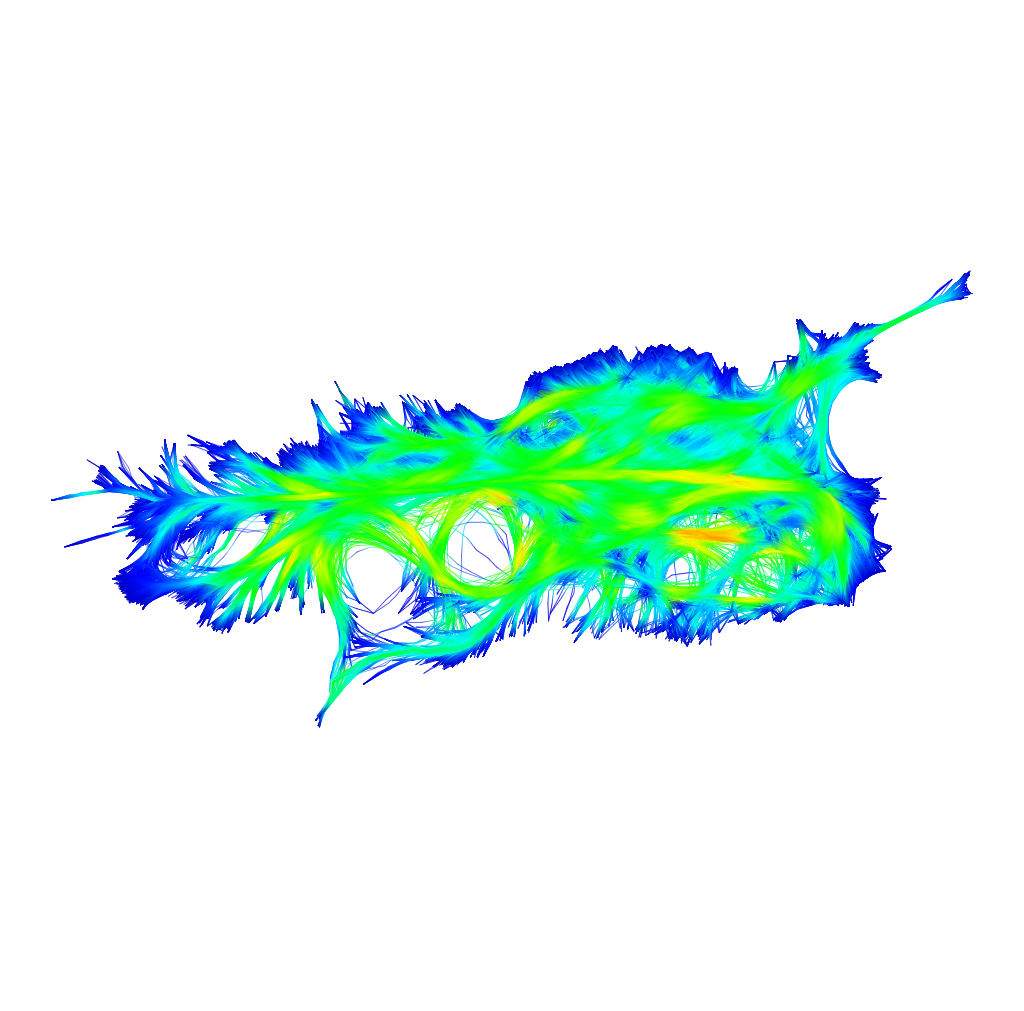
\includegraphics[width=0.48\linewidth]{rjmr-allicds/city-ibavb-40its-1eps-ambiguity.png}}
\subfloat[IBAVB 40its]{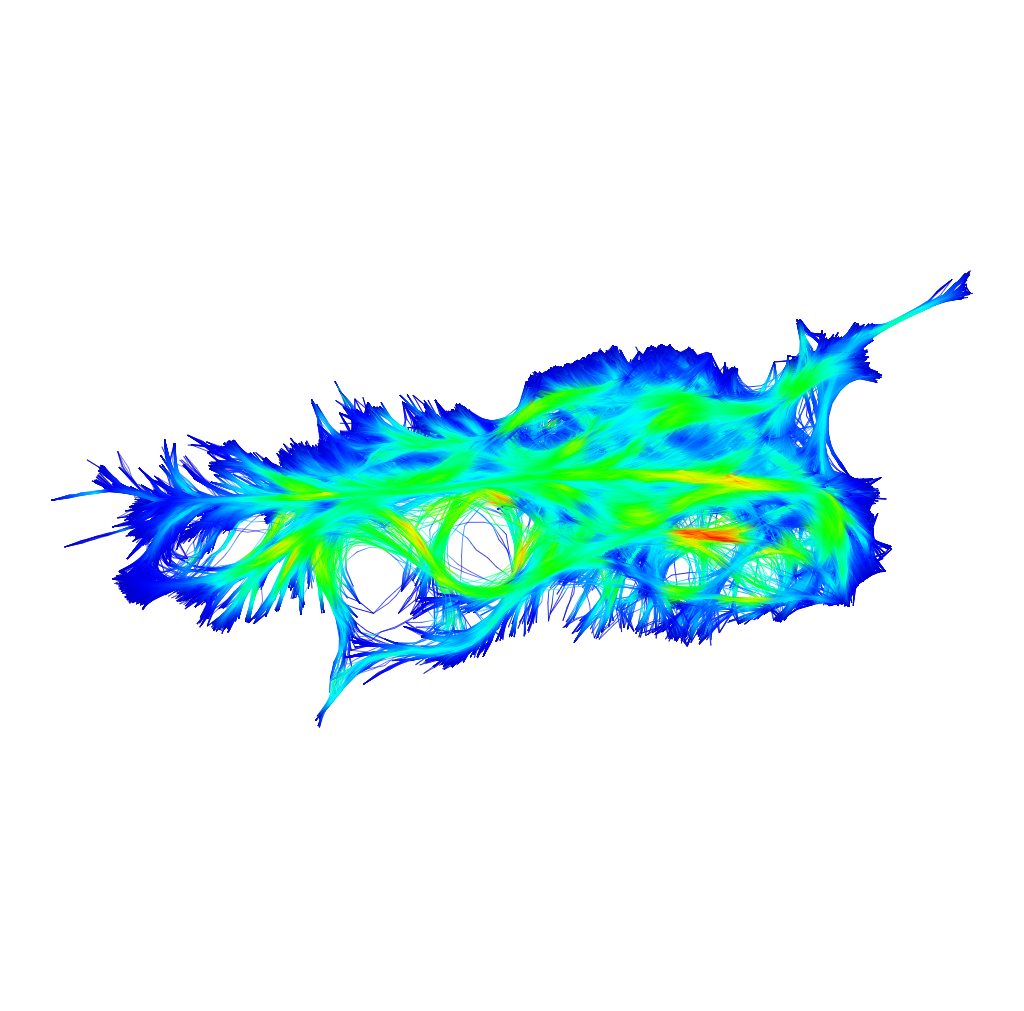
\includegraphics[width=0.48\linewidth]{rjmr-allicds/city-ibavb-40its-1eps-ambiguity-relative.png}} \\
\subfloat[IBAVB 40its]{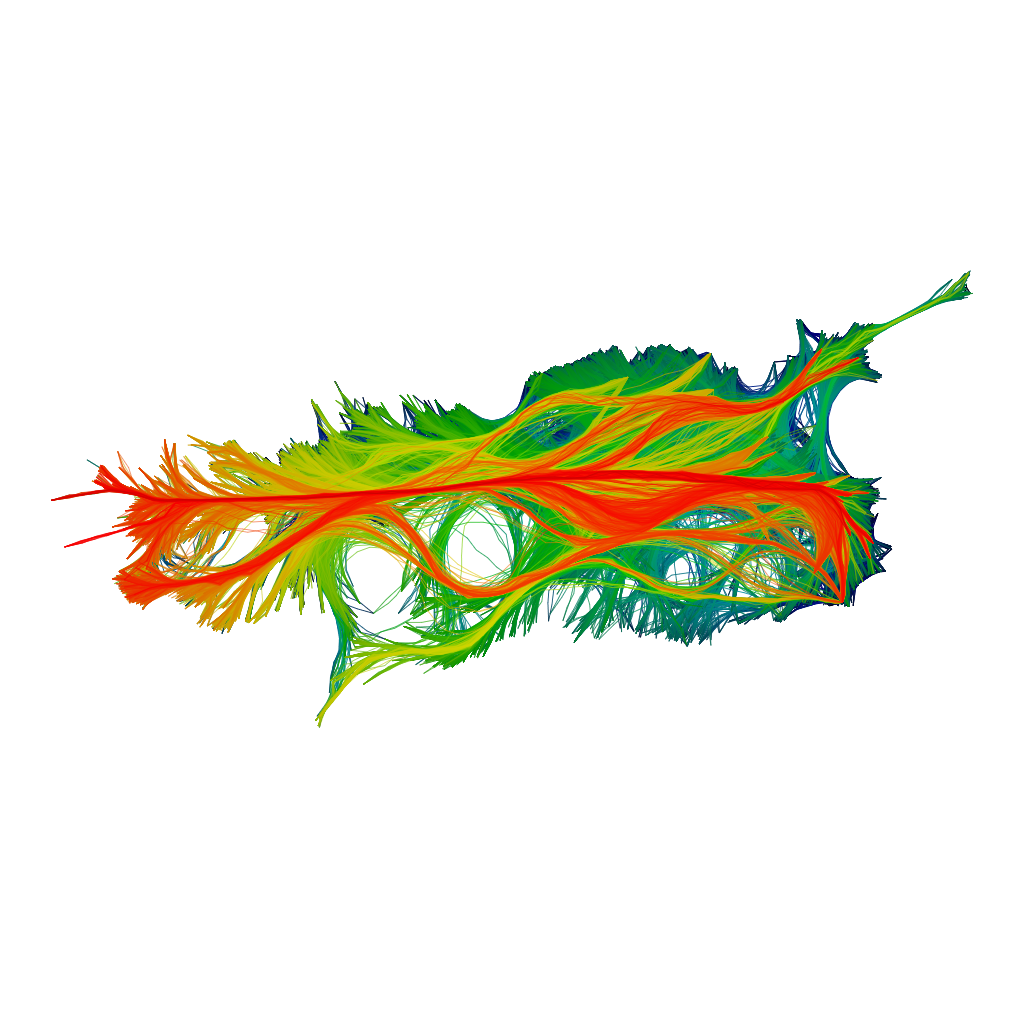
\includegraphics[width=0.48\linewidth]{rjmr-allicds/city-ibavb-40its-1eps-edgelength.png}}
\end{figure}

\begin{figure}[ht]
\centering
\subfloat[CUBu]{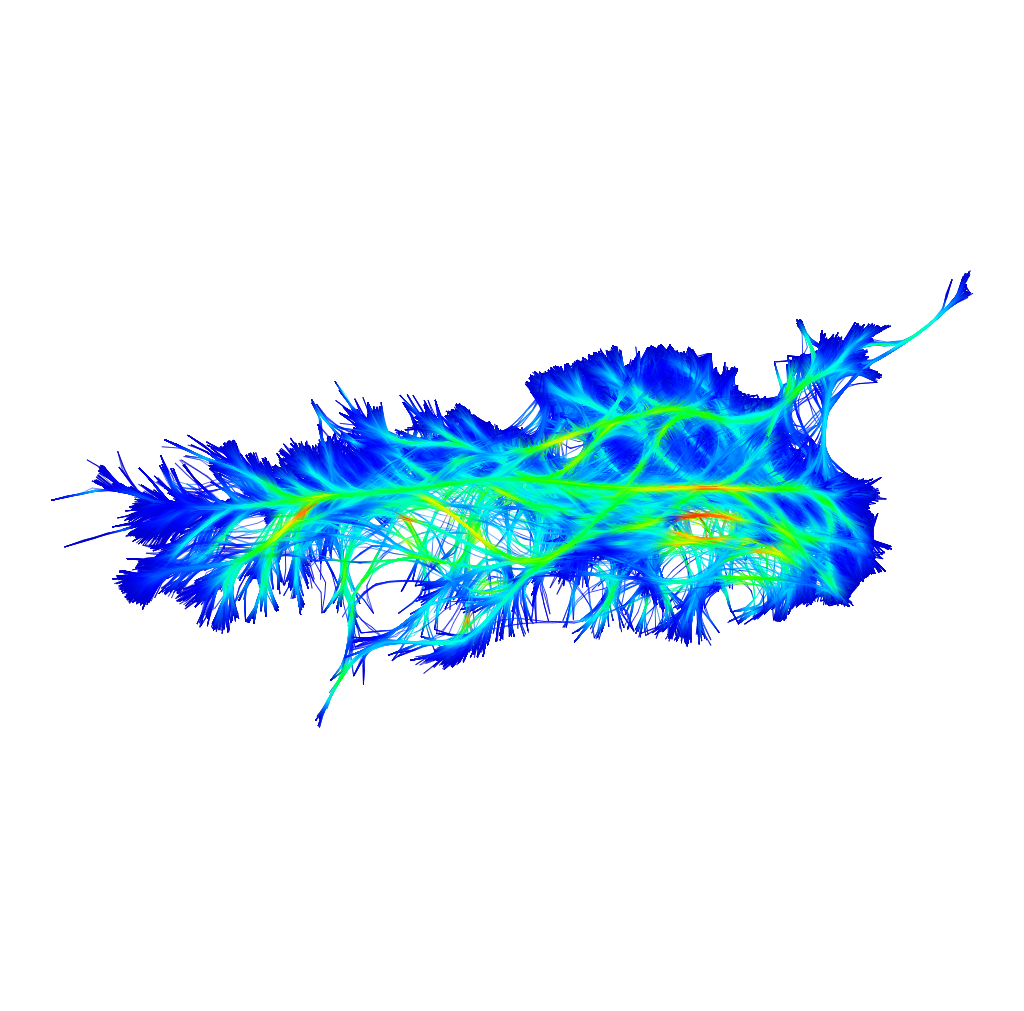
\includegraphics[width=0.48\linewidth]{rjmr-allicds/city-cubu-ambiguity-relative.png}}\\
\subfloat[CUBu]{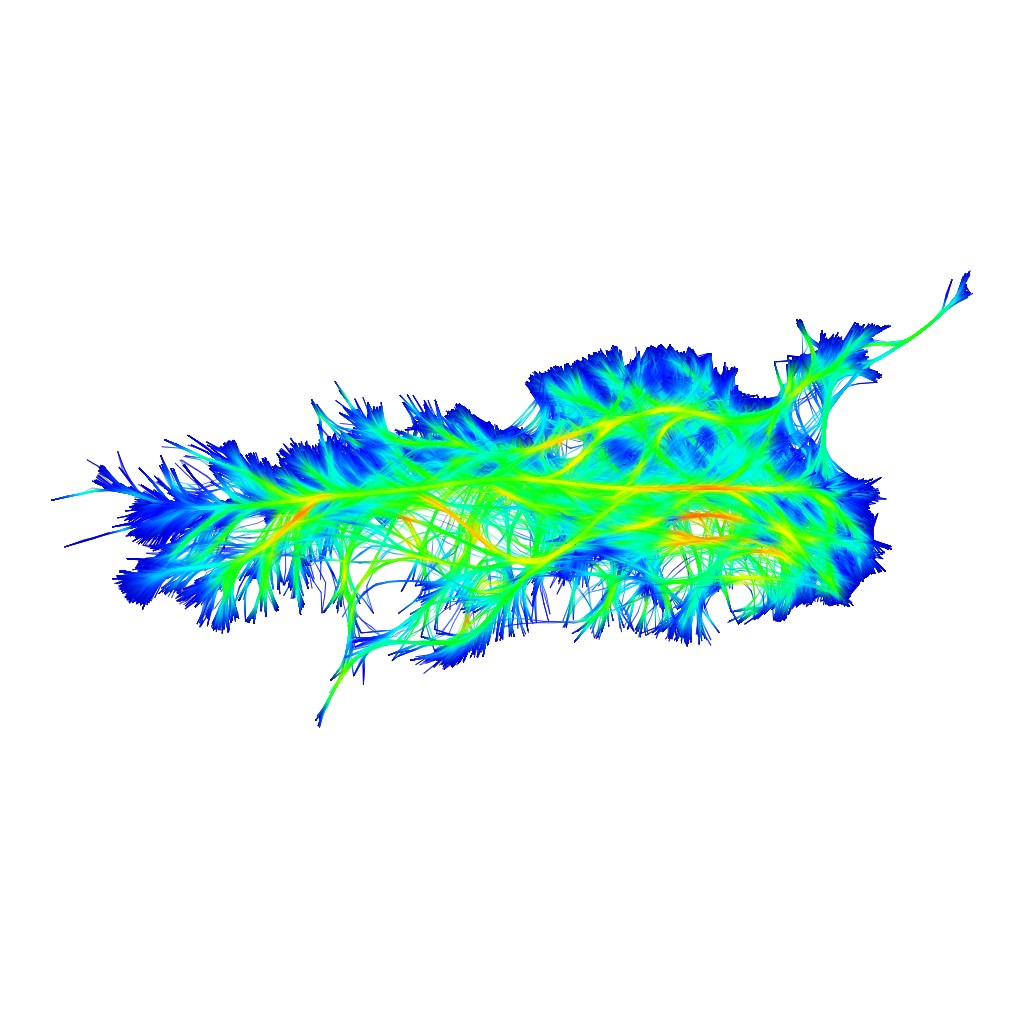
\includegraphics[width=0.48\linewidth]{rjmr-allicds/city-cubu-ambiguity.png}}
\subfloat[CUBu]{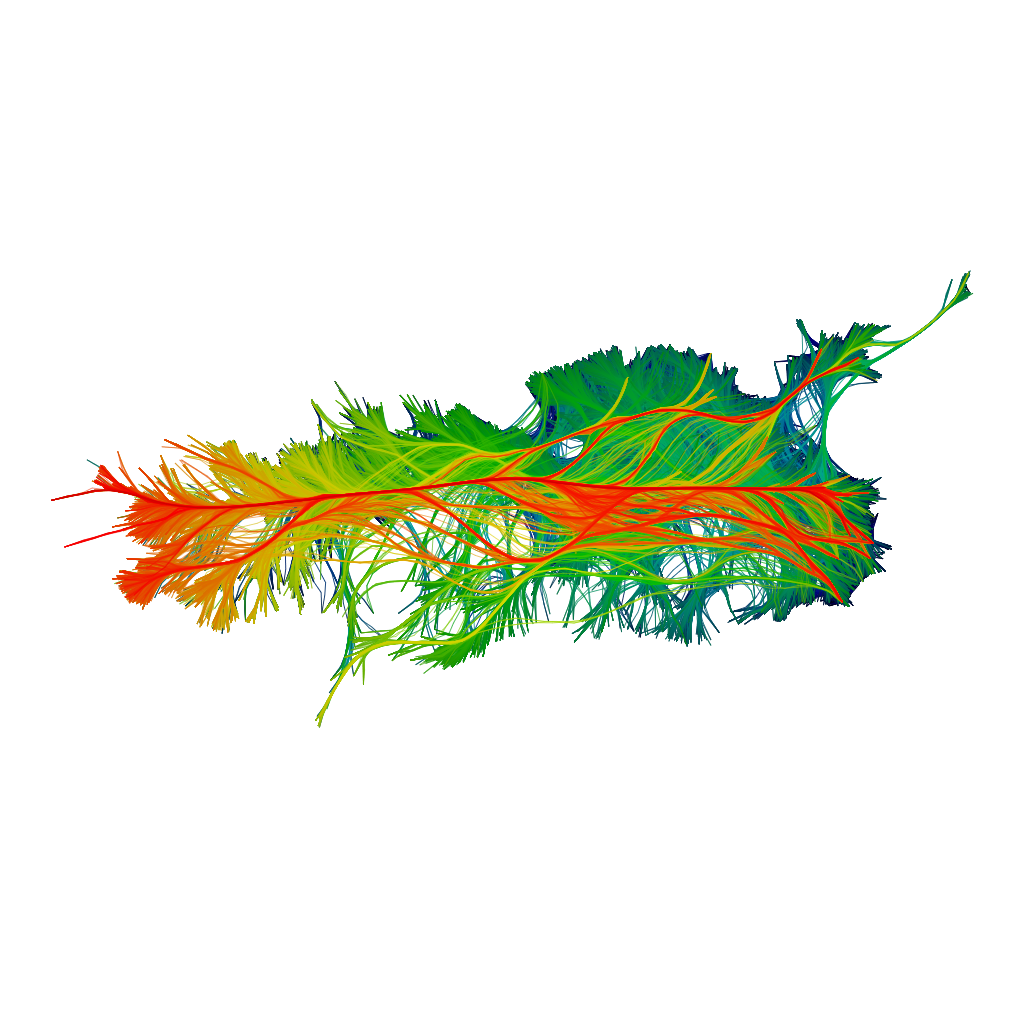
\includegraphics[width=0.48\linewidth]{rjmr-allicds/city-cubu-edgelength.png}}\\
\caption{Rio de Janeiro Metropolitan Region: all procedures 2019/2020}
\end{figure}

\clearpage

%!TeX root=../paper.tex

\section{Discussion}\label{sec:discussion}

Building upon the results presented in the previous section, we now discuss the key aspects of the proposed method, including its performance in avoiding ambiguity, its flexibility, computational performance, and limitations.

\subsection{Flexibility}

By operating as an additional layer on existing iterative bundling algorithms, IBAVB inherits the characteristics of the underlying method. This approach leverages existing bundling literature to adapt to the specific requirements of a given problem, allowing IBAVB to be implemented on top of the most suitable bundling technique. While IBAVB is limited to iterative methods, this is not a significant restriction, as most state-of-the-art bundling techniques, particularly image-based methods, are iterative in nature\cite{lhuillier:2017:survey}. This modular design ensures compatibility with ongoing developments in iterative bundling; consequently, improvements in bundle formation or specialized case management within these algorithms directly enhance IBAVB's performance.


\subsection{Ambiguity-Avoidance}

IBAVB demonstrates superior performance in ambiguity avoidance compared to existing methods, effectively preventing the formation of visually confusing bundle intersections. From our tests, it outperforms both traditional bundling methods and Edge Path Bundling for ambiguity avoidance. However, this improvement in ambiguity comes with a notable trade-off in terms of overall bundle quality. Our approach tends to have increased visual clutter. This trade-off between ambiguity avoidance and visual density represents a fundamental characteristic of our approach.

\subsection{Limitations}\label{sec:limitations}

While our proposed metric offers a valuable tool for assessing and reducing ambiguity in bundling, it is important to acknowledge its inherent limitations. These limitations primarily concern computational performance and scope of application.

\textbf{Computational Cost:}

IBAVB's core visualization method is extremely simple and computationally efficient, as we only read from a texture and modulate a vector according to it. However, computing $\omega$ presents several computational challenges. The na\"ive implementation without approximations has substantial VRAM consumption and exhibits prohibitively slow computation times, making it infeasible for practical use. We mitigated this issue through the proposed approximation and pre-computation of the paths differences. For offline computation and analysis tasks, the performance is satisfactory. Our approximated implementation successfully handles offline rendering of visualizations with millions of paths on consumer-grade hardware, demonstrating IBAVB's practical applicability. However, real-time rendering is a constraint, which does not impact the method's primary use case. We argue that this computational trade-off is well justified, as IBAVB represents a significant advancement in ambiguity-avoiding bundling methods for trail visualization.

IBAVB's core visualization method is extremely simple and computationally efficient, as we only read from a texture and modulate a vector according to it. However, computing $\omega$ presents computational challenges due to high VRAM consumption and architectural limitations on GPUs. We have successfully addressed these through strategic approximations and pre-computation techniques. The only remaining performance constraint is real-time rendering, which does not impact the method's primary use case. In fact, our approximated implementation successfully handles offline rendering of visualizations with millions of paths on consumer-grade hardware, demonstrating IBAVB's practical applicability. This computational trade-off is well justified, as IBAVB represents a significant advancement in ambiguity-avoiding bundling methods for trail visualization.

% lucas: IDK if this is something that we should _really_ set as a limitation. Often the non-iterative methods use only the structure of the network to bundle and thus aim to not be ambiguous in the first place (at least indirectly). Therefore, I don't think there's a significant lack of impact because of this.
\textbf{Applicability to Bundling Algorithms:} IBAVB is currently designed to function specifically with iterative bundling algorithms. While iterative techniques represent a significant portion of existing bundling methods, this design choice limits IBAVB's applicability to other bundling paradigms, such as hierarchical approaches. This restriction affects the tool's versatility across the full spectrum of bundling techniques.

\textbf{Bundle Formation Optimization:} Our approach operates based on local information, modulating whether or not to bundle edges and how much to do so. It does not directly influence how edges are bundled. Consequently, while our metric can prevent undesirable bundling, it does not guarantee optimal bundle formation. This limitation could result in bundles that are locally improved but globally suboptimal. It also leads to increase visual clutter compared to the default techniques IBAVB is built upon.

%!TeX root=../paper.tex

\section{Conclusion}\label{sec:conclusion}

In this paper, we introduced a novel metric ($\omega$) for measuring local ambiguity in bundled path visualizations, and IBAVB, an ambiguity-aware bundling method that builds upon existing iterative bundling techniques. Our metric addresses a significant gap in the field by providing localized measurements of ambiguity throughout the visualization, allowing for more precise evaluation and control of bundle clarity. Through extensive validation, we demonstrated that $\omega$ effectively captures ambiguity patterns across various scenarios, from simple crossings to complex bundle configurations.

IBAVB leverages the capabilities of $\omega$ to create bundled visualizations that actively avoid high-ambiguity configurations. By modulating the bundling process based on local ambiguity measurements, our method achieves improved visual clarity while maintaining the benefits of path bundling. The method's design as an extension to existing iterative bundling algorithms ensures its broad applicability and allows it to inherit the specific advantages of different bundling techniques.

While our current implementation presents some computational limitations for real-time applications, it performs well for offline visualization tasks, successfully handling millions of paths on consumer-grade hardware. Future work could explore optimization strategies to improve real-time performance and extend the method's applicability to non-iterative bundling paradigms.


\bibliographystyle{IEEEtran}
\bibliography{bib}

% You can manually copy in the resultant .bbl file and set second argument of $\backslash${\tt{begin}} to the number of references
%  (used to reserve space for the reference number labels box).

% \begin{thebibliography}{1}
% \bibliographystyle{IEEEtran}

% \bibitem{ref1}
% {\it{Mathematics Into Type}}. American Mathematical Society. [Online]. Available: https://www.ams.org/arc/styleguide/mit-2.pdf

% \bibitem{ref2}
% T. W. Chaundy, P. R. Barrett and C. Batey, {\it{The Printing of Mathematics}}. London, U.K., Oxford Univ. Press, 1954.

% \bibitem{ref3}
% F. Mittelbach and M. Goossens, {\it{The \LaTeX Companion}}, 2nd ed. Boston, MA, USA: Pearson, 2004.

% \bibitem{ref4}
% G. Gr\"atzer, {\it{More Math Into LaTeX}}, New York, NY, USA: Springer, 2007.

% \bibitem{ref5}M. Letourneau and J. W. Sharp, {\it{AMS-StyleGuide-online.pdf,}} American Mathematical Society, Providence, RI, USA, [Online]. Available: http://www.ams.org/arc/styleguide/index.html

% \bibitem{ref6}
% H. Sira-Ramirez, ``On the sliding mode control of nonlinear systems,'' \textit{Syst. Control Lett.}, vol. 19, pp. 303--312, 1992.

% \bibitem{ref7}
% A. Levant, ``Exact differentiation of signals with unbounded higher derivatives,''  in \textit{Proc. 45th IEEE Conf. Decis.
% Control}, San Diego, CA, USA, 2006, pp. 5585--5590. DOI: 10.1109/CDC.2006.377165.

% \bibitem{ref8}
% M. Fliess, C. Join, and H. Sira-Ramirez, ``Non-linear estimation is easy,'' \textit{Int. J. Model., Ident. Control}, vol. 4, no. 1, pp. 12--27, 2008.

% \bibitem{ref9}
% R. Ortega, A. Astolfi, G. Bastin, and H. Rodriguez, ``Stabilization of food-chain systems using a port-controlled Hamiltonian description,'' in \textit{Proc. Amer. Control Conf.}, Chicago, IL, USA,
% 2000, pp. 2245--2249.
% \end{thebibliography}

\newpage

% \section{Biography Section}
% If you have an EPS/PDF photo (graphicx package needed), extra braces are
%  needed around the contents of the optional argument to biography to prevent
%  the LaTeX parser from getting confused when it sees the complicated
%  $\backslash${\tt{includegraphics}} command within an optional argument. (You can create
%  your own custom macro containing the $\backslash${\tt{includegraphics}} command to make things
%  simpler here.)
%  
% \vspace{11pt}

% \bf{If you include a photo:}\vspace{-33pt}
% \begin{IEEEbiography}[{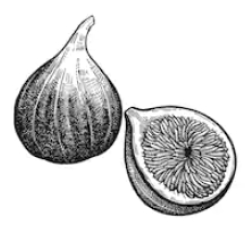
\includegraphics[width=1in,height=1.25in,clip,keepaspectratio]{fig1}}]{Michael Shell}
% Use $\backslash${\tt{begin\{IEEEbiography\}}} and then for the 1st argument use $\backslash${\tt{includegraphics}} to declare and link the author photo.
% Use the author name as the 3rd argument followed by the biography text.
% \end{IEEEbiography}

% \vspace{11pt}

% \bf{If you will not include a photo:}\vspace{-33pt}
% \begin{IEEEbiographynophoto}{John Doe}
% Use $\backslash${\tt{begin\{IEEEbiographynophoto\}}} and the author name as the argument followed by the biography text.
% \end{IEEEbiographynophoto}


\vfill

\end{document}
